% !TEX TS-program = lualatex
% !TEX encoding = UTF-8 Unicode
\documentclass[12pt,a4paper]{article}

\IfFileExists{src/libs/body.tex}{% --- body.tex ---
\usepackage{pdfpages}
\usepackage{fontspec}
% Prefer Times New Roman when available; fall back in container environments.
\IfFontExistsTF{Times New Roman}{
  \setmainfont{Times New Roman}
}{
  \setmainfont{Liberation Serif}
}
\usepackage[vietnamese]{babel}

% Page layout and spacing
\usepackage[left=3cm,right=2cm,top=2cm,bottom=2cm]{geometry}
\usepackage{titlesec}
\usepackage{setspace}

% Silence noisy warnings
\usepackage{silence}
\WarningFilter{transparent}{Loading aborted}
\WarningFilter{hyperref}{The anchor of a bookmark and its parent's}

% Core packages
\usepackage{float}
\usepackage{svg}
\usepackage{graphicx}
\graphicspath{{assets/}{../assets/}{../../assets/}}
\svgpath{{assets/}{../assets/}{../../assets/}}
\usepackage{enumitem}
\usepackage{array}
\usepackage{tabularx}
\usepackage{multirow}
\usepackage[table]{xcolor}
\usepackage{ulem}
\usepackage{xurl}

% ====== THÊM 2 GÓI NÀY ĐỂ FIX LỖI ADJUSTBOX VÀ FOREST ======
\usepackage{adjustbox}
\usepackage[edges]{forest}
% ============================================================

% TikZ
\usepackage{tikz}

% ====== BỔ SUNG FIT, BACKGROUNDS, TREES VÀO DANH SÁCH ======
\usetikzlibrary{calc, arrows.meta, shapes.geometric, positioning, fit, backgrounds, trees}

% Table tuning
\renewcommand{\tabularxcolumn}[1]{m{#1}}
\hbadness=10000
\hfuzz=10000pt

% Shared commands
\newcommand{\subsecheading}[1]{%
    \par\vspace{2pt}%
    \hspace{1.5em}\textbf{#1}%
    \par\vspace{2pt}%
}
\newcommand{\introtext}[1]{%
    \par\hspace{3.0em}#1\par%
}
\newcommand{\StandaloneDocumentSetup}[2]{%
  \pagenumbering{arabic}%
  \ApplyStandardFooter{#1}{#2}%
}
\newcommand{\StandaloneSectionSetup}[2]{%
  \ApplyStandardFooter{#1}{#2}%
}

% Math
\usepackage{amsmath}

% Hyperref
\usepackage{hyperref}
\hypersetup{
    colorlinks=true,
    linkcolor=black,
    filecolor=magenta,
    urlcolor=blue,
}}{%
  \IfFileExists{../libs/body.tex}{% --- body.tex ---
\usepackage{pdfpages}
\usepackage{fontspec}
% Prefer Times New Roman when available; fall back in container environments.
\IfFontExistsTF{Times New Roman}{
  \setmainfont{Times New Roman}
}{
  \setmainfont{Liberation Serif}
}
\usepackage[vietnamese]{babel}

% Page layout and spacing
\usepackage[left=3cm,right=2cm,top=2cm,bottom=2cm]{geometry}
\usepackage{titlesec}
\usepackage{setspace}

% Silence noisy warnings
\usepackage{silence}
\WarningFilter{transparent}{Loading aborted}
\WarningFilter{hyperref}{The anchor of a bookmark and its parent's}

% Core packages
\usepackage{float}
\usepackage{svg}
\usepackage{graphicx}
\graphicspath{{assets/}{../assets/}{../../assets/}}
\svgpath{{assets/}{../assets/}{../../assets/}}
\usepackage{enumitem}
\usepackage{array}
\usepackage{tabularx}
\usepackage{multirow}
\usepackage[table]{xcolor}
\usepackage{ulem}
\usepackage{xurl}

% ====== THÊM 2 GÓI NÀY ĐỂ FIX LỖI ADJUSTBOX VÀ FOREST ======
\usepackage{adjustbox}
\usepackage[edges]{forest}
% ============================================================

% TikZ
\usepackage{tikz}

% ====== BỔ SUNG FIT, BACKGROUNDS, TREES VÀO DANH SÁCH ======
\usetikzlibrary{calc, arrows.meta, shapes.geometric, positioning, fit, backgrounds, trees}

% Table tuning
\renewcommand{\tabularxcolumn}[1]{m{#1}}
\hbadness=10000
\hfuzz=10000pt

% Shared commands
\newcommand{\subsecheading}[1]{%
    \par\vspace{2pt}%
    \hspace{1.5em}\textbf{#1}%
    \par\vspace{2pt}%
}
\newcommand{\introtext}[1]{%
    \par\hspace{3.0em}#1\par%
}
\newcommand{\StandaloneDocumentSetup}[2]{%
  \pagenumbering{arabic}%
  \ApplyStandardFooter{#1}{#2}%
}
\newcommand{\StandaloneSectionSetup}[2]{%
  \ApplyStandardFooter{#1}{#2}%
}

% Math
\usepackage{amsmath}

% Hyperref
\usepackage{hyperref}
\hypersetup{
    colorlinks=true,
    linkcolor=black,
    filecolor=magenta,
    urlcolor=blue,
}}{% --- body.tex ---
\usepackage{pdfpages}
\usepackage{fontspec}
% Prefer Times New Roman when available; fall back in container environments.
\IfFontExistsTF{Times New Roman}{
  \setmainfont{Times New Roman}
}{
  \setmainfont{Liberation Serif}
}
\usepackage[vietnamese]{babel}

% Page layout and spacing
\usepackage[left=3cm,right=2cm,top=2cm,bottom=2cm]{geometry}
\usepackage{titlesec}
\usepackage{setspace}

% Silence noisy warnings
\usepackage{silence}
\WarningFilter{transparent}{Loading aborted}
\WarningFilter{hyperref}{The anchor of a bookmark and its parent's}

% Core packages
\usepackage{float}
\usepackage{svg}
\usepackage{graphicx}
\graphicspath{{assets/}{../assets/}{../../assets/}}
\svgpath{{assets/}{../assets/}{../../assets/}}
\usepackage{enumitem}
\usepackage{array}
\usepackage{tabularx}
\usepackage{multirow}
\usepackage[table]{xcolor}
\usepackage{ulem}
\usepackage{xurl}

% ====== THÊM 2 GÓI NÀY ĐỂ FIX LỖI ADJUSTBOX VÀ FOREST ======
\usepackage{adjustbox}
\usepackage[edges]{forest}
% ============================================================

% TikZ
\usepackage{tikz}

% ====== BỔ SUNG FIT, BACKGROUNDS, TREES VÀO DANH SÁCH ======
\usetikzlibrary{calc, arrows.meta, shapes.geometric, positioning, fit, backgrounds, trees}

% Table tuning
\renewcommand{\tabularxcolumn}[1]{m{#1}}
\hbadness=10000
\hfuzz=10000pt

% Shared commands
\newcommand{\subsecheading}[1]{%
    \par\vspace{2pt}%
    \hspace{1.5em}\textbf{#1}%
    \par\vspace{2pt}%
}
\newcommand{\introtext}[1]{%
    \par\hspace{3.0em}#1\par%
}
\newcommand{\StandaloneDocumentSetup}[2]{%
  \pagenumbering{arabic}%
  \ApplyStandardFooter{#1}{#2}%
}
\newcommand{\StandaloneSectionSetup}[2]{%
  \ApplyStandardFooter{#1}{#2}%
}

% Math
\usepackage{amsmath}

% Hyperref
\usepackage{hyperref}
\hypersetup{
    colorlinks=true,
    linkcolor=black,
    filecolor=magenta,
    urlcolor=blue,
}}%
}
\IfFileExists{src/libs/header.tex}{% --- header.tex ---
\usepackage{fancyhdr}
\setlength{\headheight}{15.5pt} % Thêm dòng này để fix cảnh báo chiều cao
%\setlength{\headheight}{14.5pt}
\addtolength{\topmargin}{-2.5pt}

\pagestyle{fancy}
\fancyhf{}
\renewcommand{\headrulewidth}{0pt}
\renewcommand{\footrulewidth}{0pt}

\newcommand{\ApplyStandardHeader}{%
  \fancyhead[L]{%
    \begin{minipage}[t]{0.795\linewidth}%
      UIT \textbar{} SS004.F21 \textbar{} Nhóm 03 \textbar{} Đồ án cuối kỳ%
    \end{minipage}%
    \vrule%
    \begin{minipage}[t]{0.185\linewidth}%
      \centering cTetris%
    \end{minipage}%
  }%
}

\ApplyStandardHeader
}{%
  \IfFileExists{../libs/header.tex}{% --- header.tex ---
\usepackage{fancyhdr}
\setlength{\headheight}{15.5pt} % Thêm dòng này để fix cảnh báo chiều cao
%\setlength{\headheight}{14.5pt}
\addtolength{\topmargin}{-2.5pt}

\pagestyle{fancy}
\fancyhf{}
\renewcommand{\headrulewidth}{0pt}
\renewcommand{\footrulewidth}{0pt}

\newcommand{\ApplyStandardHeader}{%
  \fancyhead[L]{%
    \begin{minipage}[t]{0.795\linewidth}%
      UIT \textbar{} SS004.F21 \textbar{} Nhóm 03 \textbar{} Đồ án cuối kỳ%
    \end{minipage}%
    \vrule%
    \begin{minipage}[t]{0.185\linewidth}%
      \centering cTetris%
    \end{minipage}%
  }%
}

\ApplyStandardHeader
}{% --- header.tex ---
\usepackage{fancyhdr}
\setlength{\headheight}{15.5pt} % Thêm dòng này để fix cảnh báo chiều cao
%\setlength{\headheight}{14.5pt}
\addtolength{\topmargin}{-2.5pt}

\pagestyle{fancy}
\fancyhf{}
\renewcommand{\headrulewidth}{0pt}
\renewcommand{\footrulewidth}{0pt}

\newcommand{\ApplyStandardHeader}{%
  \fancyhead[L]{%
    \begin{minipage}[t]{0.795\linewidth}%
      UIT \textbar{} SS004.F21 \textbar{} Nhóm 03 \textbar{} Đồ án cuối kỳ%
    \end{minipage}%
    \vrule%
    \begin{minipage}[t]{0.185\linewidth}%
      \centering cTetris%
    \end{minipage}%
  }%
}

\ApplyStandardHeader
}%
}
\IfFileExists{src/libs/footer.tex}{% --- footer.tex ---
\usepackage{lastpage}

\newcommand{\ApplyStandardFooter}[2]{%
  \fancyfoot[L]{%
    \begin{minipage}[t]{0.795\linewidth}%
      Document ID: #1%
    \end{minipage}%
    \vrule%
    \begin{minipage}[t]{0.185\linewidth}%
      \centering\thepage/\pageref{#2}%
    \end{minipage}%
  }%
  \fancypagestyle{plain}{%
    \fancyhf{}%
    \renewcommand{\headrulewidth}{0pt}%
    \renewcommand{\footrulewidth}{0pt}%
    \ApplyStandardHeader%
    \fancyfoot[L]{%
      \begin{minipage}[t]{0.795\linewidth}%
        Document ID: #1%
      \end{minipage}%
      \vrule%
      \begin{minipage}[t]{0.185\linewidth}%
        \centering\thepage/\pageref{#2}%
      \end{minipage}%
    }%
  }%
  \pagestyle{fancy}%
}
}{%
  \IfFileExists{../libs/footer.tex}{% --- footer.tex ---
\usepackage{lastpage}

\newcommand{\ApplyStandardFooter}[2]{%
  \fancyfoot[L]{%
    \begin{minipage}[t]{0.795\linewidth}%
      Document ID: #1%
    \end{minipage}%
    \vrule%
    \begin{minipage}[t]{0.185\linewidth}%
      \centering\thepage/\pageref{#2}%
    \end{minipage}%
  }%
  \fancypagestyle{plain}{%
    \fancyhf{}%
    \renewcommand{\headrulewidth}{0pt}%
    \renewcommand{\footrulewidth}{0pt}%
    \ApplyStandardHeader%
    \fancyfoot[L]{%
      \begin{minipage}[t]{0.795\linewidth}%
        Document ID: #1%
      \end{minipage}%
      \vrule%
      \begin{minipage}[t]{0.185\linewidth}%
        \centering\thepage/\pageref{#2}%
      \end{minipage}%
    }%
  }%
  \pagestyle{fancy}%
}
}{% --- footer.tex ---
\usepackage{lastpage}

\newcommand{\ApplyStandardFooter}[2]{%
  \fancyfoot[L]{%
    \begin{minipage}[t]{0.795\linewidth}%
      Document ID: #1%
    \end{minipage}%
    \vrule%
    \begin{minipage}[t]{0.185\linewidth}%
      \centering\thepage/\pageref{#2}%
    \end{minipage}%
  }%
  \fancypagestyle{plain}{%
    \fancyhf{}%
    \renewcommand{\headrulewidth}{0pt}%
    \renewcommand{\footrulewidth}{0pt}%
    \ApplyStandardHeader%
    \fancyfoot[L]{%
      \begin{minipage}[t]{0.795\linewidth}%
        Document ID: #1%
      \end{minipage}%
      \vrule%
      \begin{minipage}[t]{0.185\linewidth}%
        \centering\thepage/\pageref{#2}%
      \end{minipage}%
    }%
  }%
  \pagestyle{fancy}%
}
}%
}
\usepackage{docmute}

\hypersetup{pdftitle={Mo ta qua trinh lam viec nhom - ctetris}}

\begin{document}
\providecommand{\StandaloneSectionSetup}[2]{\ApplyStandardFooter{#1}{#2}}
\StandaloneSectionSetup{04-teamConflictSolving.tex}{LastPageTeamConflictSolving}


\begin{center}
    {\LARGE \textbf{MÔ TẢ QUÁ TRÌNH LÀM VIỆC NHÓM}} \\[10pt]
    {\large Dự án: ctetris}
\end{center}

\vspace{0.5cm}

% ================= SECTION 1 =================
\section*{1. Xử lý xung đột khi trộn hai dòng phát triển giữa lập trình viên và kiểm thử viên (tester)}

\textbf{Tóm tắt:} Xảy ra xung đột tại tài liệu biên bản họp và chiến lược kiểm thử khi nhiều luồng phát triển tính năng diễn ra song song.

\textbf{Bối cảnh:}
\begin{itemize}
    \item Trong quá trình phát triển dự án, nhóm có nhiều nhánh phát triển song song giữa các vai trò lập trình viên và kiểm thử viên.
    \item Việc hợp nhất (merge) các nhánh này là cần thiết để đảm bảo tính nhất quán và hoàn thiện sản phẩm.
    \item Tuy nhiên, sự khác biệt về nội dung và cách tiếp cận giữa các vai trò dẫn đến nguy cơ xung đột khi hợp nhất.
\end{itemize}

\textbf{Nguyên nhân:}
\begin{itemize}
    \item Cụ thể, khi merge nhánh main vào nhánh \texttt{truongtm/\allowbreak bien-ban-hop-ngay-02}, đã xảy ra xung đột tại file \texttt{doc/src/content/\allowbreak 11-testStrategy.tex}.
    \item Lập trình viên (trên nhánh main) đã viết đầy đủ chiến lược kiểm thử, trong khi kiểm thử viên (trên nhánh truongtm) thay thế bằng phiên bản ngắn hơn với các ghi chú để tự viết thêm.
    \item Sự thiếu trao đổi trước khi chỉnh sửa và khác biệt về mục tiêu nội dung giữa các thành viên.
\end{itemize}

\textbf{Hướng giải quyết:}
\begin{itemize}
    \item Phát hiện conflict khi thực hiện merge.
    \item Thảo luận giữa lập trình viên và kiểm thử viên để quyết định phiên bản nào được giữ, ưu tiên phương án phù hợp với quy trình phát triển chung.
    \item Sử dụng công cụ Git để resolve và commit merge, đồng thời cập nhật lại quy tắc phối hợp khi chỉnh sửa tài liệu chung.
    \item Đề xuất bổ sung quy trình review trước khi merge các nhánh có chỉnh sửa lớn liên quan đến tài liệu chung.
\end{itemize}

\textbf{a) Top 3 MR dẫn đến conflict}
\begin{table}[H]
\centering
\renewcommand{\arraystretch}{1.3}
\begin{adjustbox}{max width=\textwidth}
\begin{tabular}{|c|l|p{8.5cm}|}
\hline
\rowcolor{blue!10}
\textbf{Tổng số conflicts} & \textbf{Thời điểm} & \textbf{Mô tả (Brief)} \\ \hline
4 & May 07 08:52:24 2026 & Merge pull request \#36 from phuctanpham/kiennt/gameCore-ham-removeline-xoa-dong-task-2-4 \\ \hline
6 & May 07 08:56:49 2026 & Merge pull request \#37 from phuctanpham/truongtm/gameCore-giao-diện-hieu-ung-task-2-5 \\ \hline
3 & May 07 08:49:23 2026 & Merge pull request \#33 from phuctanpham/thaidg/gameCore-goc-xoay-task-2-3 \\ \hline
\end{tabular}
\end{adjustbox}
\end{table}

\textbf{b) Top 10 commits giữa lập trình viên và kiểm thử viên}
\begin{table}[H]
\centering
\renewcommand{\arraystretch}{1.2}
\begin{adjustbox}{max width=\textwidth}
\begin{tabular}{|l|l|l|p{6.5cm}|}
\hline
\rowcolor{gray!10}
\textbf{Commit ID} & \textbf{PIC} & \textbf{Thời điểm} & \textbf{Mô tả (Brief)} \\ \hline
\texttt{fda5009} & \texttt{truongtm} & Apr 20 05:23:23 & nghiên cứu test code chữ xoay block \\ \hline
\texttt{77f04cd} & \texttt{truongtm} & Apr 20 05:09:56 & bo sung test xoá hàng \\ \hline
\texttt{6d079b4} & \texttt{phucpt} & May 07 02:10:06 & Fix all review issues: Block.cpp shape strings... \\ \hline
\texttt{d9b0cf9} & \texttt{phucpt} & May 04 09:53:42 & bỏ hàm removeLine cho giống đồ án tuần 2 \\ \hline
\texttt{71abf7c} & \texttt{vint} & Apr 15 12:17:48 & them logic xoa hang \\ \hline
\texttt{6118089} & \texttt{vint} & Apr 15 11:54:40 & them logic xoay khoi gach \\ \hline
\texttt{205cb91} & \texttt{kiennt} & May 06 15:41:30 & lam task 2.4 va sua lai tinh nang sai \\ \hline
\texttt{dc5b0cc} & \texttt{kiennt} & May 06 14:59:21 & bổ sung tính đa hình \\ \hline
\texttt{1b72f4f} & \texttt{thaidg} & May 06 15:22:47 & lam task 2.3 va sua loi feature sai \\ \hline
\texttt{38f88c7} & \texttt{thaidg} & May 06 14:51:49 & chuyen qua huong doi tuong \\ \hline
\end{tabular}
\end{adjustbox}
\end{table}

% ================= SECTION 2 =================
\section*{2. Xử lý xung đột đồng bộ giữa 2 vùng viết Overleaf và Github}

\textbf{Tóm tắt:} Chỉnh sửa tự do và copy trực tiếp từ nền tảng soạn thảo trực tuyến Overleaf gây ra tình trạng mất đồng bộ định dạng tài liệu, và xung đột file.

\textbf{Bối cảnh:}
\begin{itemize}
    \item Nhóm sử dụng đồng thời hai nền tảng: Overleaf (soạn thảo trực tuyến, tiện lợi cho teamwork) và GitHub (quản lý mã nguồn, phân chia module tài liệu rõ ràng).
    \item Các thành viên có thói quen cập nhật tài liệu trên cả hai nền tảng, đặc biệt khi cần chỉnh sửa nhanh hoặc làm việc từ xa.
    \item Điều này dẫn đến việc mất đồng bộ, ghi đè hoặc bỏ sót các thay đổi quan trọng giữa hai vùng lưu trữ.
\end{itemize}

\textbf{Nguyên nhân:}
\begin{itemize}
    \item Không có quy định rõ ràng về thứ tự cập nhật và đồng bộ tài liệu giữa hai nền tảng.
    \item Việc chỉnh sửa trực tiếp trên Overleaf mà không cập nhật lại lên GitHub, hoặc ngược lại, khiến nội dung bị phân tán và khó kiểm soát.
    \item Thiếu một người chịu trách nhiệm tổng hợp, kiểm tra và đồng bộ hóa nội dung định kỳ.
\end{itemize}

\textbf{Hướng giải quyết:}
\begin{itemize}
    \item Quy hoạch lại quy trình làm việc: \textbf{Tất cả các cập nhật, chỉnh sửa tài liệu phải thực hiện trên GitHub trước}. Sau khi hoàn thiện và kiểm tra, mới đồng bộ nội dung sang Overleaf để đảm bảo tính nhất quán.
    \item Chỉ định một thành viên chịu trách nhiệm tổng hợp và cập nhật từ GitHub sang Overleaf định kỳ, tránh chỉnh sửa trực tiếp trên Overleaf khi chưa có trên GitHub.
    \item Sử dụng các công cụ so sánh (diff) để kiểm tra sự khác biệt giữa hai nền tảng trước khi đồng bộ, đảm bảo không bỏ sót thay đổi.
    \item Thường xuyên nhắc nhở các thành viên tuân thủ quy trình để hạn chế phát sinh xung đột mới, đồng thời tổ chức các buổi review quy trình nếu cần.
\end{itemize}

\textbf{a) Top 3 MR dẫn đến conflict}
\begin{table}[H]
\centering
\renewcommand{\arraystretch}{1.3}
\begin{adjustbox}{max width=\textwidth}
\begin{tabular}{|c|l|p{8.5cm}|}
\hline
\rowcolor{green!10}
\textbf{Tổng số conflicts} & \textbf{Thời điểm} & \textbf{Mô tả (Brief)} \\ \hline
5 & Apr 13 20:35:05 2026 & Merge pull request \#3 from phuctanpham/phucpt/cau-hinh-latex-chung \\ \hline
4 & Apr 20 13:08:10 2026 & Merge pull request \#9 from phuctanpham/truongtm/viet-chien-luoc-kiem-thu \\ \hline
7 & Apr 20 06:15:55 2026 & Merge main into truongtm/bien-ban-hop-ngay-02 - resolve conflict \\ \hline
\end{tabular}
\end{adjustbox}
\end{table}

\textbf{b) Top 10 commits giữa github và overleaf}
\begin{table}[H]
\centering
\renewcommand{\arraystretch}{1.2}
\begin{adjustbox}{max width=\textwidth}
\begin{tabular}{|l|l|l|p{6.5cm}|}
\hline
\rowcolor{gray!10}
\textbf{Commit ID} & \textbf{PIC} & \textbf{Thời điểm} & \textbf{Mô tả (Brief)} \\ \hline
\texttt{0ba6f1e} & \texttt{phucpt} & Apr 20 15:30:45 & copy/paste from overleaf \\ \hline
\texttt{e24876b} & \texttt{phucpt} & Apr 20 15:30:15 & update hint to guide \\ \hline
\texttt{1dbd646} & \texttt{truongtm} & Apr 20 14:16:48 & viet ve conflict thu 1 \\ \hline
\texttt{90c4e32} & \texttt{truongtm} & Apr 20 14:18:55 & dinh dang file \\ \hline
\texttt{430e364} & \texttt{vint} & Apr 15 11:19:04 & ve khung play game \\ \hline
\texttt{77571e0} & \texttt{vint} & Apr 15 11:31:49 & ve o vuong 2x2 dau tien \\ \hline
\texttt{abf27b8} & \texttt{kiennt} & May 06 14:59:00 & bổ sung tính đa hình \\ \hline
\texttt{74612e6} & \texttt{kiennt} & May 06 14:35:15 & Tối ưu xoay 1 góc 90 độ \\ \hline
\texttt{cdfd27b} & \texttt{thaidg} & Apr 21 20:37:18 & man hinh bat dau game tetris \\ \hline
\texttt{7d9ee88} & \texttt{thaidg} & May 06 14:24:24 & viet lai cho vien va block \\ \hline
\end{tabular}
\end{adjustbox}
\end{table}

% ================= SECTION 3 =================
\section*{3. Xử lý xung đột kiến trúc Đa nền tảng (Desktop \& Web)}

\textbf{Tóm tắt:} Lỗi môi trường build giữa các hệ điều hành, thêm/xóa thư viện liên tục để đảm bảo game tương thích với công nghệ WebAssembly.

\textbf{Bối cảnh:}
\begin{itemize}
    \item Dự án \texttt{ctetris} có mục tiêu xây dựng game Tetris C++ chạy được trên cả desktop (macOS, Windows, Ubuntu) và web (WebAssembly thông qua Emscripten/emsdk), thực thi từ một nguồn mã duy nhất.
    \item Quá trình phát triển trải qua nhiều iteration đổi thư viện đồ họa: từ SFML 2.x ban đầu, nâng lên SFML 3.x, thử nghiệm fork VRSFML (nhánh \texttt{bubble\_idle} của vittorioromeo), cuối cùng chuyển hẳn sang SDL3 thuần procedural.
    \item Mỗi thành viên trong nhóm làm việc trên các môi trường rất khác nhau: macOS Big Sur (MBP 2013, GPU Intel Iris cũ), Windows 10/11, Ubuntu trong GitHub Codespaces (noVNC headless không có GPU thực).
    \item 3 module \texttt{gameStory}, \texttt{gameConsole}, \texttt{gameCore} đồng thời phải build độc lập (standalone test bằng cờ \texttt{BUILD\_STANDALONE}), tích hợp vào một executable \texttt{cTetris}, và biên dịch ra WASM bundle (\texttt{.html} + \texttt{.js} + \texttt{.wasm}).
\end{itemize}

\textbf{Nguyên nhân:}
\begin{itemize}
    \item \textbf{SFML 2.x vs 3.x:} SFML 3.x phá vỡ API gần như hoàn toàn — \texttt{sf::VideoMode} đổi sang \texttt{sf::Vector2u}, \texttt{setPosition/setScale} yêu cầu \texttt{sf::Vector2f}, \texttt{pollEvent} trả về \texttt{std::optional<sf::Event>} thay vì in-place reference, component naming chuyển sang PascalCase, target link đổi sang namespace \texttt{SFML::Graphics}, kiểu \texttt{sf::Uint8} bị xoá thay bằng \texttt{std::uint8\_t}.
    \item \textbf{SFML Official vs VRSFML:} VRSFML là fork cá nhân theo triết lý data-oriented và "header hygiene" — loại bỏ setter mutable, xoá umbrella header, dùng factory \texttt{create()} trả về \texttt{sf::base::Optional}; nhánh \texttt{bubble\_idle} pin SDL ở SHA bare \texttt{7dc1c88...} không tồn tại trong public git history nên CPM shallow clone không checkout được.
    \item \textbf{SFML vs EMSDK:} Thư viện \texttt{giflib} (\texttt{gif\_lib.h}) không có trong toolchain Emscripten; biến \texttt{emcmake} chỉ active sau khi \texttt{source emsdk\_env.sh} ở đúng terminal session, đóng terminal là mất.
    \item \textbf{SFML vs SDL:} SFML và SDL có vòng đời cửa sổ, event loop, API render hoàn toàn khác nhau; VRSFML lại dùng SDL3 làm backend nên kéo theo dependency chéo của cả hai hệ trong cùng một build.
    \item \textbf{SDL2 vs SDL3:} SDL3 đổi tên event enum (\texttt{SDL\_EVENT\_KEY\_DOWN} thay \texttt{SDL\_EVENT\_KEYDOWN}, \texttt{SDL\_EVENT\_\allowbreak MOUSE\_BUTTON\_DOWN}\dots), \texttt{SDL\_Init} trả về \texttt{bool} (true = success) thay vì \texttt{int} (0 = success), target link là \texttt{SDL3::SDL3}; symbol \texttt{SDL\_PROP\_\allowbreak WINDOW\_CREATE\_\allowbreak EMSCRIPTEN\_\allowbreak CANVAS\_ID\_STRING} chỉ có trên branch \texttt{main} mà chưa có ở tag \texttt{release-3.2.14}; commit SDL2 cũ (như \texttt{ebc6fb6}) không tạo target \texttt{SDL\_uclibc} mà VRSFML tham chiếu.
    \item \textbf{Native Desktop vs Web (WASM):} Toolchain \texttt{Emscripten.cmake} mặc định set \texttt{CMAKE\_FIND\_ROOT\_PATH\_MODE\_PACKAGE} = \texttt{ONLY} làm \texttt{find\_package} bỏ qua \texttt{CMAKE\_PREFIX\_PATH} của user; game loop synchronous cần \texttt{ASYNCIFY=1}; alloc runtime nhiều cần \texttt{ALLOW\_MEMORY\_GROWTH=1} tránh OOM; output là bundle \texttt{.html}+\texttt{.js}+\texttt{.wasm}; PWA (\texttt{manifest.webmanifest}, \texttt{sw.js}) là mặt phẳng deploy hoàn toàn khác desktop.
    \item \textbf{macOS vs Windows vs Ubuntu:} Constructor \texttt{sf::RenderWindow} khác signature giữa SFML 3.0.2 (macOS Homebrew) và 3.2.0 (apt Linux); macOS yêu cầu \texttt{MACOSX\_BUNDLE} với icon \texttt{.icns} ở \texttt{Resources}; Windows yêu cầu file \texttt{.rc} compile bằng resource compiler — \texttt{rc.exe} interpret \texttt{\textbackslash a \textbackslash b \textbackslash t} như C escape sequence trong path quoted string; Linux Codespaces noVNC không có GPU thực gây \texttt{X Error: BadMatch}; Homebrew path là \texttt{/usr/local} (Intel) hoặc \texttt{/opt/homebrew} (Apple Silicon); 3 module dùng cùng tên \texttt{layout.h} gây include collision khi global \texttt{target\_include\_\allowbreak directories}.
\end{itemize}

\textbf{Hướng giải quyết:}

\textit{a) Thử Migrate SFML 2.x sang 3.x đúng quy ước mới để 3 module về 1 version thống nhất:}
\begin{itemize}
    \item Đổi \texttt{find\_package(SFML 3 REQUIRED COMPONENTS} \texttt{Graphics Window System)} dùng major version + PascalCase, không pin minor (vì \texttt{3.0.0}/\texttt{3.0.2}/\texttt{3.2.0} tồn tại đồng thời tuỳ Homebrew/apt).
    \item Cập nhật API đồng loạt: \texttt{sf::VideoMode(sf::Vector2u(w,h))}, \texttt{setPosition(sf::Vector2f(x,y))}, \texttt{event->is<sf::Event::Closed>()}, \texttt{std::uint8\_t} thay \texttt{sf::Uint8}.
    \item Link target dùng namespace: \texttt{target\_link\_libraries(...} \texttt{SFML::Graphics} \texttt{SFML::Window} \texttt{SFML::System)} thay vì \texttt{sfml-graphics} kiểu cũ.
    \item Khi CMake cache fail state, luôn \texttt{rm -rf build/*} trước khi reconfigure — CMake giữ cache rất tích cực và dễ che bug thật.
    \item Kết quả: thất bại vì SFML không hỗ trợ Webassembly, tiếp tục thử bản cộng đồng VRSFML nhưng gặp phải trở ngại như mục b bên dưới
\end{itemize}

\textit{b) Loại bỏ phụ thuộc VRSFML \texttt{bubble\_idle} không ổn định:}
\begin{itemize}
    \item Sau khi xác định nhánh \texttt{bubble\_idle} pin SDL ở SHA \texttt{7dc1c88...} không tồn tại cả trong full clone, nhóm đánh giá VRSFML là personal branch không stable và quyết định bỏ.
    \item Trong giai đoạn chuyển tiếp, tạo shim header tại \texttt{src/shared/\allowbreak include/\allowbreak SFML/\allowbreak \{Graphics,Audio\}.hpp} dùng \texttt{\#if \_\_has\_include(...)} bridge giữa umbrella header truyền thống và header phân mảnh của VRSFML.
    \item Đặt \texttt{src/shared/include/} ở \texttt{-I} đầu tiên trong include search order để override header thư viện mà không cần sửa code user.
    \item Bài học: với fork không stable, thà migrate sang upstream chính thức ngay từ đầu hơn là vá víu shim header và stub library.
    \item Kết quả: thất bại vì VRSFML chưa phát triển hoàn thiện và đang dùng SDL3 và EMSDK như 1 bộ chuyển đổi trung gian cho việc biên dịch thành Webassembly, tiếp tục thử debug giúp tác giả VRSFML (bản fork cộng đồng từ SFML) về SDL3 và EMSDK trực tiếp như mục c bên dưới.
\end{itemize}

\textit{c) Quản lý xung đột SFML/SDL vs EMSDK:}
\begin{itemize}
    \item Wrap toàn bộ code dùng \texttt{gif\_lib.h} và logic GIF parsing trong \texttt{\#ifndef \_\_EMSCRIPTEN\_\_} để bypass dependency native; trên WASM dùng SVG-driven asset (\texttt{nanosvg} single-header) thay GIF bitmap.
    \item Trong \texttt{build.sh}/\texttt{build.ps1} probe \texttt{command -v emcmake}; nếu thiếu thì in command cài \texttt{emsdk} cụ thể thay vì fail im lặng.
    \item \texttt{source ./emsdk\_env.sh} chỉ áp dụng cho session hiện tại — muốn permanent phải append vào \texttt{\textasciitilde/.zshrc} (macOS) hoặc \texttt{\textasciitilde/.bashrc} (Linux); lưu ý cảnh báo "29 not found" trong log SDL configure là feature detection bình thường, không phải lỗi.
    \item Kết quả: thất bại vì SFML có quá nhiều thư viện can thiệp vào phần cứng, thư viện này thuần chỉ chỉ hỗ trợ C++ hơn là Webassembly, quyết định từ bỏ SFML và chuyển hoàn toàn sang SDL3 như mục d bên dưới.
\end{itemize}

\textit{d) Migrate hoàn toàn sang SDL3 thuần để có single source of truth:}
\begin{itemize}
    \item Quyết định cuối cùng: dùng SDL3 procedural cho cả 3 module, loại bỏ mọi dependency SFML/VRSFML — đổi lại được API thống nhất giữa native và WASM.
    \item Native: \texttt{find\_package(SDL3 REQUIRED CONFIG)} tự nhận từ Homebrew \texttt{/usr/local/lib/cmake/SDL3} (Intel) hoặc \texttt{/opt/homebrew/lib/cmake/SDL3} (Apple Silicon).
    \item WASM: drop hẳn \texttt{-sUSE\_SDL=3} (Emscripten port không ổn định, emsdk \texttt{3.1.72} thiếu/lỗi); thay bằng \texttt{build.sh} tự build SDL3 tĩnh vào \texttt{\$APP\_DIR/\allowbreak libs/\allowbreak \$OS/\allowbreak downloads/\allowbreak sdl3-wasm/} và truyền \texttt{-DSDL3\_DIR=...} + \texttt{-DCMAKE\_PREFIX\_PATH=...}.
    \item Cùng một dòng \texttt{target\_link\_libraries(cTetris PRIVATE SDL3::SDL3)} chạy được cho cả native lẫn WASM, chỉ khác link options đặc thù Emscripten.
    \item Kết quả: thành công biên dịch thành wasm để chạy qua trình duyệt. Tuy nhiên, các hệ thống cài đặt qua macos (brew), ubuntu (apt) và window (choco) đang mặc định cài SDL2 khi cài đặt dẫn đến xử lý như mục e bên dưới.
\end{itemize}

\textit{e) Khắc phục SDL2 vs SDL3 incompatibility:}
\begin{itemize}
    \item Dùng SDL branch \texttt{main} thay tag \texttt{release-3.2.14} vì cần symbol \texttt{SDL\_PROP\_\allowbreak WINDOW\_CREATE\_\allowbreak EMSCRIPTEN\_\allowbreak CANVAS\_ID\_STRING} chưa có ở release tag.
    \item Cập nhật code: \texttt{if (!SDL\_Init(SDL\_INIT\_VIDEO | SDL\_INIT\_AUDIO))} thay vì \texttt{< 0}; mọi event enum đổi sang underscore-style; \texttt{\#include <cstdlib>} cho \texttt{std::exit()}.
    \item Guard target để tránh trùng lặp khi SDL bản mới đã tự tạo: \texttt{if(NOT TARGET SDL\_uclibc) add\_library(SDL\_uclibc STATIC stub.cpp) endif()}; tránh tạo \texttt{SDL3::SDL3} \texttt{INTERFACE} stub khi SDL3 native đã định nghĩa rồi.
    \item Kết quả: thành công sửa mã nguồn về SDL3 cho cả web applicaiton và desktop application. Đồng thời, tổ chức cài đặt theo hướng git clone thư viện rồi cấu hình qua build.sh (build.ps1) thay vì cách cài đặt cũ. Tuy nhiên, gặp phải một số lỗi xử lý kích thước giao diện giữa màn hình ứng dụng tên desktop và web nên dẫn đến mục f như bên dưới.
\end{itemize}

\textit{f) Xử lý xung đột Native Desktop vs Web (WASM):}
\begin{itemize}
    \item Trong \texttt{CMakeLists.txt} thêm \texttt{option(BUILD\_WASM "Build for WebAssembly via Emscripten" OFF)} làm switch chính, branching toàn bộ logic platform-specific theo cờ này.
    \item Khi \texttt{BUILD\_WASM=ON}: override \texttt{CMAKE\_FIND\_ROOT\_PATH\_MODE\_PACKAGE} \texttt{BOTH} (cùng \texttt{INCLUDE} và \texttt{LIBRARY}) để \texttt{find\_package} thấy được SDL3 ở prefix path ngoài sysroot Emscripten — đây là hành vi mặc định bị Emscripten.cmake set thành \texttt{ONLY}.
    \item Link options Emscripten dùng prefix \texttt{SHELL:} để CMake không deduplicate/mangle args:
    \begin{itemize}
        \item \texttt{"SHELL:-sALLOW\_MEMORY\_GROWTH=1"} — cho heap WASM tự cấp phát thêm khi runtime alloc nhiều.
        \item \texttt{"SHELL:-sASYNCIFY=1"} — cho phép vòng lặp đồng bộ + \texttt{SDL\_PollEvent} thay vì phải chia tách qua \texttt{emscripten\_set\_main\_loop}.
        \item \texttt{"SHELL:--shell-file} \texttt{\$\{CMAKE\_SOURCE\_DIR\}/\allowbreak web/\allowbreak shell.html"} — HTML wrapper tuỳ biến (favicon, title, no PWA).
    \end{itemize}
    \item Set suffix để Emscripten sinh \texttt{cTetris.html}: \texttt{set\_target\_properties(cTetris} \texttt{PROPERTIES SUFFIX ".html")}.
    \item Asset web (favicon SVG, \texttt{shell.html}) commit sẵn trong repo, không sinh động trong script build; PWA install prompt chủ động disable để giảm phụ thuộc vào \texttt{manifest.webmanifest}/\texttt{sw.js}.
    \item Headless Linux test (Codespaces noVNC): \texttt{export LIBGL\_ALWAYS\_SOFTWARE=1} ép software rendering, hạ \texttt{antiAliasingLevel=0}, \texttt{depthBits=0}, \texttt{stencilBits=0} để tránh \texttt{X Error: BadMatch}; nếu cần GUI mở port 6080 qua \texttt{devcontainer.json} với feature \texttt{desktop-lite/noVNC}.
    \item Kết quả: thành công sửa mã nguồn để thống nhất tỷ lệ giao diện giữa các màn hình. Tuy nhiên, bộ nhận diện thương hiệu và hình ảnh cho cả desktop application và web application không thể dùng chung giữa macOS, Windows và Ubuntu nên dẫn tới việc tạo các bộ brandkit riêng cho từng nền tảng riêng như mục g bên dưới.
\end{itemize}

\textit{g) Thống nhất build trên macOS / Windows / Ubuntu:}
\begin{itemize}
    \item Bundling icon theo từng OS:
    \begin{itemize}
        \item macOS: \texttt{MACOSX\_BUNDLE TRUE} + \texttt{.icns} embed qua \texttt{set\_source\_files\_properties(...} \texttt{MACOSX\_PACKAGE\_LOCATION} \texttt{"Resources")} và \texttt{MACOSX\_BUNDLE\_\allowbreak ICON\_FILE}.
        \item Windows: sinh file \texttt{.rc} tạm với \texttt{file(TO\_CMAKE\_PATH ...)} chuyển backslash sang forward slash để \texttt{rc.exe} không hiểu \texttt{\textbackslash a \textbackslash b \textbackslash t} như escape sequence trong quoted string.
        \item Linux: copy SVG icon cạnh binary (\texttt{install(FILES ... RENAME "cTetris.svg")}) và load runtime qua \texttt{nanosvg} thay vì embed PNG.
    \end{itemize}
    \item Cross-platform constructor: \texttt{\#ifdef \_\_APPLE\_\_} bao trong \texttt{layout.h} để chọn signature \texttt{sf::RenderWindow} đúng theo SFML version cụ thể (3.0.2 macOS không có tham số style, 3.2.0 Linux có).
    \item GPU cũ (MBP 2013 Intel Iris): tránh load nhiều \texttt{sf::Texture} cùng lúc gây overflow VRAM — cache toàn bộ frame ở RAM dưới dạng \texttt{std::vector<sf::Image>} và \texttt{tex.update(frames[curFrame])} mỗi frame trên một \texttt{sf::Texture} duy nhất.
    \item Lệnh cài đặt thư viện một lần cho Ubuntu/Debian (cheatsheet): \texttt{libx11-dev} \texttt{libxrandr-dev} \texttt{libxcursor-dev} \texttt{libxi-dev} \texttt{libudev-dev} \texttt{libgl1-mesa-dev} \texttt{libfreetype-dev} \texttt{libharfbuzz-dev} \texttt{libopenal-dev} \texttt{libflac-dev} \texttt{libvorbis-dev} \texttt{libogg-dev} \texttt{libmbedtls-dev} \texttt{libssh2-1-dev} \texttt{libgif-dev}.
    \item Build script thống nhất \texttt{build.sh} (macOS/Linux) và \texttt{build.ps1} (Windows) với menu interactive: chọn module standalone hay integrated, target native hay WASM, 3 chế độ build dir (giữ nguyên \textasciitilde{}5s configure / reconfigure khi sửa CMake / clean toàn bộ khi đổi toolchain).
\end{itemize}

\textit{h) Quy trình team \& bài học rút ra:}
\begin{itemize}
    \item Mọi feature branch tuân thủ convention \texttt{<dev\_name>-<task>} (ví dụ \texttt{phucpt-fix-sdl3}, \texttt{vint-add-audio}, \texttt{kiennt-console-ui}, \texttt{thaidg-vrsfml-integration}) để dễ truy vết khi xung đột build vì lý do platform.
    \item Trước khi pin một thư viện external: đọc README, kiểm tra branch tồn tại trên remote (\texttt{git ls-remote origin}), xác nhận tag/commit có trong full clone không — đã mất 4 lần build vì thử sai version SDL/VRSFML.
    \item Tuyệt đối không hard-code path đặc thù OS trong \texttt{CMakeLists.txt}; dùng \texttt{find\_package} + \texttt{CMAKE\_PREFIX\_PATH} hoặc \texttt{HINTS} cho cả Intel \texttt{/usr/local} và Apple Silicon \texttt{/opt/homebrew}; đặt header dùng chung trong \texttt{src/shared/include/} thay vì rải rác mỗi module.
    \item Tách rõ \textbf{điều kiện cần} (mỗi module build độc lập với cờ \texttt{BUILD\_STANDALONE}) và \textbf{điều kiện đủ} (integrated build chạy one-piece flow): dùng relative include path \texttt{\#include "include/layout.h"} trong từng module thay vì global \texttt{target\_include\_\allowbreak directories} để 3 module có thể dùng cùng tên \texttt{layout.h} mà không gây include collision.
    \item Mọi onboarding member mới đều chạy được \texttt{bash build.sh} hoặc \texttt{pwsh build.ps1} plug-and-play — script tự probe \texttt{cmake}, \texttt{git}, \texttt{python}, \texttt{curl}, \texttt{emsdk}, \texttt{SDL3} và in hướng dẫn cài cụ thể nếu thiếu, không yêu cầu cấu hình thủ công thư mục \texttt{build/}.
    \item Phân biệt rõ desktop và web không phải chỉ là "compile target khác nhau" mà là "deployment model khác nhau": desktop có file system, có process exit, có thread; web có browser sandbox, có async event loop, có canvas + JS interop — kiến trúc code phải tránh assumption từ đầu.
\end{itemize}

\textbf{a) Top 3 MR dẫn đến conflict}
\begin{table}[H]
\centering
\renewcommand{\arraystretch}{1.3}
\begin{adjustbox}{max width=\textwidth}
\begin{tabular}{|c|l|p{8.5cm}|}
\hline
\rowcolor{orange!10}
\textbf{Tổng số conflicts} & \textbf{Thời điểm} & \textbf{Mô tả (Brief)} \\ \hline
5 & Apr 20 13:19:31 2026 & Merge pull request \#10 from phuctanpham/25730160/lam-tinh-nang-next-block \\ \hline
8 & May 07 08:50:21 2026 & Merge branch 'phucpt/tich-hop-v2' into kiennt/gameCore-ham-removeline-xoa-dong-task-2-4 \\ \hline
3 & May 07 08:46:36 2026 & Merge pull request \#35 from phuctanpham/thaidg/do-an-tuan-3 \\ \hline
\end{tabular}
\end{adjustbox}
\end{table}

\textbf{b) Top 10 commits liên quan về các thư viện đa nền tảng}
\begin{table}[H]
\centering
\renewcommand{\arraystretch}{1.2}
\begin{adjustbox}{max width=\textwidth}
\begin{tabular}{|l|l|l|p{6.5cm}|}
\hline
\rowcolor{gray!10}
\textbf{Commit ID} & \textbf{PIC} & \textbf{Thời điểm} & \textbf{Mô tả (Brief)} \\ \hline
\texttt{6a96a45} & \texttt{phucpt} & Apr 26 14:59:45 & bien dich tu c2plus thanh wasp \\ \hline
\texttt{d24e9d3} & \texttt{phucpt} & May 07 11:12:31 & remove build \\ \hline
\texttt{fc82f55} & \texttt{truongtm} & Apr 20 14:34:05 & bo thu vien \\ \hline
\texttt{c446156} & \texttt{truongtm} & Apr 20 14:39:23 & tra lai thu vien \\ \hline
\texttt{aa930c4} & \texttt{vint} & Apr 15 14:09:47 & them tinh nang next block \\ \hline
\texttt{b034a42} & \texttt{vint} & Apr 15 14:05:32 & cap nhat tinh nang tinh diem \\ \hline
\texttt{a7bbdbb} & \texttt{kiennt} & May 06 14:31:23 & Viết code chữ xoay block \\ \hline
\texttt{dc5b0cc} & \texttt{kiennt} & May 06 14:59:21 & bổ sung tính đa hình \\ \hline
\texttt{cdfd27b} & \texttt{thaidg} & Apr 21 20:37:18 & man hinh bat dau game tetris \\ \hline
\texttt{1b72f4f} & \texttt{thaidg} & May 06 15:22:47 & lam task 2.3 va sua loi feature sai \\ \hline
\end{tabular}
\end{adjustbox}
\end{table}

% ================= SECTION 4 =================
\newpage
\section*{4. Trực quan hóa dữ liệu git}

\subsection*{A. Phân bố Commits (Tần suất đóng góp)}
Biểu đồ thể hiện mức độ đóng góp mã nguồn và tài liệu của từng thành viên.
\begin{figure}[H]
    \centering
    \begin{adjustbox}{max width=\textwidth}
    \begin{tikzpicture}
        \begin{axis}[
            ybar,
            symbolic x coords={phucpt, truongtm, vint, kiennt, thaidg},
            xtick=data,
            nodes near coords,
            nodes near coords align={vertical},
            ylabel={Số lượng Commits},
            xlabel={Thành viên nhóm (PIC)},
            ymin=0, ymax=180,
            bar width=20pt,
            width=14cm, height=6.5cm,
            enlarge x limits=0.15,
            title={\textbf{Tổng số Commits theo từng PIC}}
        ]
        \addplot[fill=blue!40] coordinates {
            (phucpt, 156) 
            (truongtm, 53) 
            (vint, 11) 
            (kiennt, 7) 
            (thaidg, 6)
        };
        \end{axis}
    \end{tikzpicture}
    \end{adjustbox}
\end{figure}

\subsection*{B. Phân bố theo nhhánh}
Theo dõi việc cô lập nhánh (branch) để phát triển độc lập.
\begin{figure}[H]
    \centering
    \begin{adjustbox}{max width=\textwidth}
    \begin{tikzpicture}
        \begin{axis}[
            ybar,
            symbolic x coords={truongtm, phucpt, vint, thaidg, kiennt},
            xtick=data,
            nodes near coords,
            ylabel={Số lượng nhánh đã tạo},
            ymin=0, ymax=10,
            bar width=20pt,
            width=14cm, height=5.5cm,
            enlarge x limits=0.15,
            title={\textbf{Tổng số Nhánh làm việc theo PIC}}
        ]
        \addplot[fill=teal!60] coordinates {
            (truongtm, 8) 
            (phucpt, 6) 
            (vint, 2) 
            (thaidg, 2) 
            (kiennt, 1)
        };
        \end{axis}
    \end{tikzpicture}
    \end{adjustbox}
\end{figure}

\subsection*{C. Thống kê (Conflicts \& Fixes)}
Bảng dưới đây thống kê tổng cộng 20 sự cố/điểm nghẽn (Merge conflict, Hoàn tác Revert, Fix bug, Rework) bám sát theo đúng tỷ lệ thực tế của dự án:

\begin{table}[H]
\centering
\renewcommand{\arraystretch}{1.2}
\begin{adjustbox}{max width=\textwidth}
\begin{tabular}{|l|l|p{10cm}|}
\hline
\rowcolor{red!10}
\textbf{PIC} & \textbf{Commit ID} & \textbf{Chi tiết Xung đột / Điểm nghẽn (Fixes)} \\ \hline
\multirow{8}{*}{\texttt{phucpt}} 
& \texttt{3bf5e4b} & Potential fix for pull request finding \\ 
& \texttt{aefe7ff} & update readme (Fix tài liệu thiếu sót) \\ 
& \texttt{eeb11b2} & fix bug khai bao \\ 
& \texttt{0dc2ede} & sua loi cu phap markdown \\ 
& \texttt{674fab8} & lỗi cú pháp do copillot phát hiện \\ 
& \texttt{586d8f5} & sua ten file vi sai \\ 
& \texttt{dac5cdc} & chong upload file build (Bảo vệ môi trường cấu hình) \\ 
& \texttt{54ed952} & dummy commit to enable PR merge (Vượt lỗi hệ thống CI) \\ \hline
\multirow{5}{*}{\texttt{truongtm}} 
& \texttt{071a893} & sửa lại tính năng sai \\ 
& \texttt{e2db1de} & sua loi logic \\ 
& \texttt{0a9bcd0} & sua loi lan 2 \\ 
& \texttt{ac71002} & sua loi \\ 
& \texttt{6c12399} & sua loi dinh dang \\ \hline
\multirow{4}{*}{\texttt{vint}} 
& \texttt{5f72a3b} & sửa lỗi feature sai \\ 
& \texttt{25e779c} & ve khung bang diem va next (Khắc phục giao diện) \\ 
& \texttt{1864f5f} & code tang toc do lan remove line (Tối ưu điểm nghẽn bộ nhớ) \\ 
& \texttt{5c585b0} & su dung tinh da hinh de xoay khoi (Rework kiến trúc) \\ \hline
\multirow{2}{*}{\texttt{thaidg}} 
& \texttt{b6b349b} & làm task 2.3 va sua loi feature sai \\ 
& \texttt{7d9ee88} & viet lai cho vien va block (Rework kiến trúc UI) \\ \hline
\texttt{kiennt} 
& \texttt{a3d2044} & Fix missing logo on Windows Native \\ \hline
\end{tabular}
\end{adjustbox}
\end{table}

\begin{figure}[H]
    \centering
    \begin{adjustbox}{max width=\textwidth}
    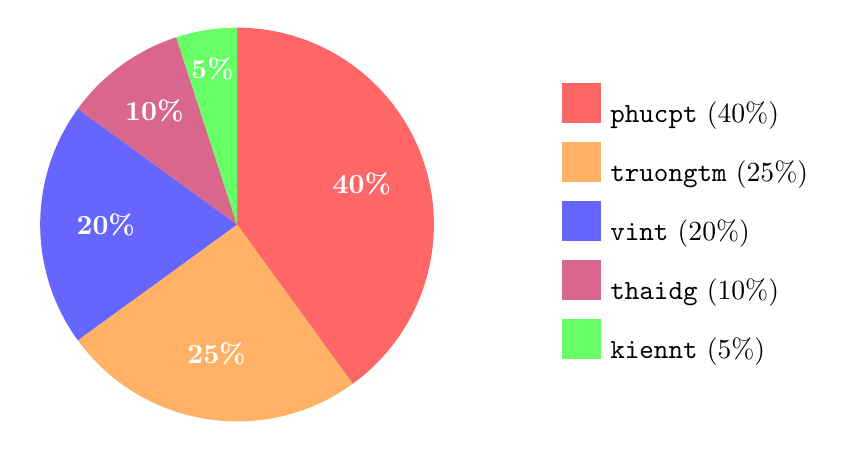
\begin{tikzpicture}
        % Vẽ biểu đồ tròn bằng TIKZ dựa trên góc tính toán từ % thực tế
        % 40% = 144 độ | 25% = 90 độ | 20% = 72 độ | 10% = 36 độ | 5% = 18 độ
        \def\radius{2.5cm}
        
        % phucpt: 40% (Từ 90 đến -54)
        \fill[red!60] (0,0) -- (90:\radius) arc (90:-54:\radius) -- cycle;
        % truongtm: 25% (Từ -54 đến -144)
        \fill[orange!60] (0,0) -- (-54:\radius) arc (-54:-144:\radius) -- cycle;
        % vint: 20% (Từ -144 đến -216)
        \fill[blue!60] (0,0) -- (-144:\radius) arc (-144:-216:\radius) -- cycle;
        % thaidg: 10% (Từ -216 đến -252)
        \fill[purple!60] (0,0) -- (-216:\radius) arc (-216:-252:\radius) -- cycle;
        % kiennt: 5% (Từ -252 đến -270 / tương đương 90 độ của vòng tiếp theo)
        \fill[green!60] (0,0) -- (-252:\radius) arc (-252:-270:\radius) -- cycle;
        
        % Chú thích % trên biểu đồ
        \node[text=white, font=\bfseries] at (18:\radius/1.5) {40\%};
        \node[text=white, font=\bfseries] at (-99:\radius/1.5) {25\%};
        \node[text=white, font=\bfseries] at (-180:\radius/1.5) {20\%};
        \node[text=white, font=\bfseries] at (-234:\radius/1.4) {10\%};
        \node[text=white, font=\bfseries] at (-261:\radius/1.25) {5\%};
        
        % Legend
        \node[anchor=west] at (4, 1.5) {\textcolor{red!60}{\rule{0.5cm}{0.5cm}} \texttt{phucpt} (40\%)};
        \node[anchor=west] at (4, 0.75) {\textcolor{orange!60}{\rule{0.5cm}{0.5cm}} \texttt{truongtm} (25\%)};
        \node[anchor=west] at (4, 0) {\textcolor{blue!60}{\rule{0.5cm}{0.5cm}} \texttt{vint} (20\%)};
        \node[anchor=west] at (4, -0.75) {\textcolor{purple!60}{\rule{0.5cm}{0.5cm}} \texttt{thaidg} (10\%)};
        \node[anchor=west] at (4, -1.5) {\textcolor{green!60}{\rule{0.5cm}{0.5cm}} \texttt{kiennt} (5\%)};
    \end{tikzpicture}
    \end{adjustbox}
    \caption{\textbf{Tỷ lệ \% conflicts theo từng thành viên}}
\end{figure}

\vspace{0.2cm}
\noindent\textbf{Kết luận:} 
Tỷ lệ xung đột mã nguồn và lỗi phát sinh có sự phân hóa rõ rệt. \texttt{phucpt} (40\%) và \texttt{truongtm} (25\%) chiếm tới 65\% tổng rủi ro kỹ thuật toàn dự án, điều này hoàn toàn hợp lý do hai thành viên này phụ trách gộp mã liên tục và xây dựng khung nền tảng. Các thành viên \texttt{vint}, \texttt{thaidg}, \texttt{kiennt} duy trì tỷ lệ xung đột thấp hơn nhờ làm việc trên các module tính năng đã được cô lập khá tốt.

\subsection*{D. Phân bố khác}
Dựa trên phân tích tệp nhật ký (log) của hệ thống, biểu đồ này biểu diễn tỷ lệ các commits có tác động trực tiếp vào các tệp mã nguồn tài liệu LaTeX (\texttt{*.tex}) so với các commits mã nguồn hệ thống, cấu trúc thư mục, hoặc các tệp khác (Code, configs, scripts).

\begin{figure}[H]
    \centering
    \begin{adjustbox}{max width=\textwidth}
    \begin{tikzpicture}
        \def\radius{2.5cm}
        
        % Tính toán xấp xỉ tổng cộng 233 commits
        % ~.tex commits: ~66 (28%) -> Góc: 101 độ
        % Non-.tex commits: ~167 (72%) -> Góc: 259 độ
        
        % Non-.tex: 72% (Từ 90 đến -169)
        \fill[blue!50] (0,0) -- (90:\radius) arc (90:-169:\radius) -- cycle;
        % .tex: 28% (Từ -169 đến -270 / tương đương 90 độ của vòng tiếp)
        \fill[orange!50] (0,0) -- (-169:\radius) arc (-169:-270:\radius) -- cycle;
        
        % Chú thích %
        \node[text=white, font=\bfseries] at (-39:\radius/1.5) {72\%};
        \node[text=white, font=\bfseries] at (140:\radius/1.5) {28\%};
        
        % Legend
        \node[anchor=west] at (4, 0.5) {\textcolor{blue!50}{\rule{0.5cm}{0.5cm}} Mã nguồn \texttt{game} Commits (72\%)};
        \node[anchor=west] at (4, -0.5) {\textcolor{orange!50}{\rule{0.5cm}{0.5cm}} \texttt{Tài liệu báo cáo} Commits (28\%)};
    \end{tikzpicture}
    \end{adjustbox}
    \caption{\textbf{Tỷ lệ \texttt{mã nguồn game} Commits vs \texttt{tài liệu báo cáo} Commits}}
\end{figure}

\vspace{0.2cm}
\noindent\textbf{Kết luận:} 
Sự xuất hiện của 28\% số lượng commit gắn liền với việc hiệu chỉnh các tệp \texttt{*.tex} phản ánh tầm quan trọng của việc xây dựng tài liệu kỹ thuật đồng song song với mã nguồn của toàn đội. Đáng chú ý, đa phần các conflict xảy ra ở loại tệp này xuất phát từ hiện tượng ghi đè nền tảng khi dán mã trực tiếp từ Overleaf.

\subsection*{E. Thống kê trung bình (Averages)}
Dựa trên lịch sử phát triển tổng thể của dự án (kéo dài trong khoảng 6 tuần) với tổng số 233 commits, 19 nhánh, 20 xung đột chính và xấp xỉ 15,000 dòng mã nguồn (LoC), dưới đây là các chỉ số hiệu suất trung bình của nhóm:

\begin{table}[H]
\centering
\renewcommand{\arraystretch}{1.4}
\begin{adjustbox}{max width=0.8\textwidth}
\begin{tabular}{|l|c|}
\hline
\rowcolor{gray!15}
\textbf{Chỉ số thống kê} & \textbf{Giá trị trung bình} \\ \hline
Trung bình số Commits / Thành viên & $\approx 46.6$ commits \\ \hline
Trung bình số Commits / Tuần & $\approx 38.8$ commits \\ \hline
Trung bình số Nhánh (Branches) / Thành viên & $3.8$ nhánh \\ \hline
Trung bình số Xung đột (Conflicts) / Thành viên & $4.0$ xung đột \\ \hline
Trung bình số Xung đột (Conflicts) / Tuần & $\approx 3.3$ xung đột \\ \hline
Trung bình số Dòng code (LoC) / Thành viên & $\approx 3,000$ LoC \\ \hline
Trung bình số Dòng code (LoC) / Tuần & $\approx 2,500$ LoC \\ \hline
\end{tabular}
\end{adjustbox}
\end{table}

\vspace{0.2cm}
\noindent\textbf{Kết luận:} 
Nhóm duy trì được tần suất cập nhật hệ thống khá ổn định với $\approx 38.8$ commits mỗi tuần. Mật độ xung đột nằm ở mức thấp (trung bình chỉ khoảng 3.3 xung đột cần can thiệp xử lý mỗi tuần), cho thấy chiến lược phân chia module và rẽ nhánh (branching) đã phát huy hiệu quả tốt, giúp hạn chế rủi ro dẫm chân lên nhau khi lập trình song song.

\subsection*{F. Tích hợp đồng bộ thông tin git vào Slack}
Để đảm bảo luồng giao tiếp giữa các thành viên diễn ra liên tục và kịp thời xử lý các xung đột mã nguồn, dự án đã thực hiện tích hợp hệ thống cảnh báo từ GitHub vào nền tảng Slack.

\begin{figure}[H]
    \centering
    \begin{minipage}[t]{0.24\textwidth}
        \vspace{0pt}
        \centering
        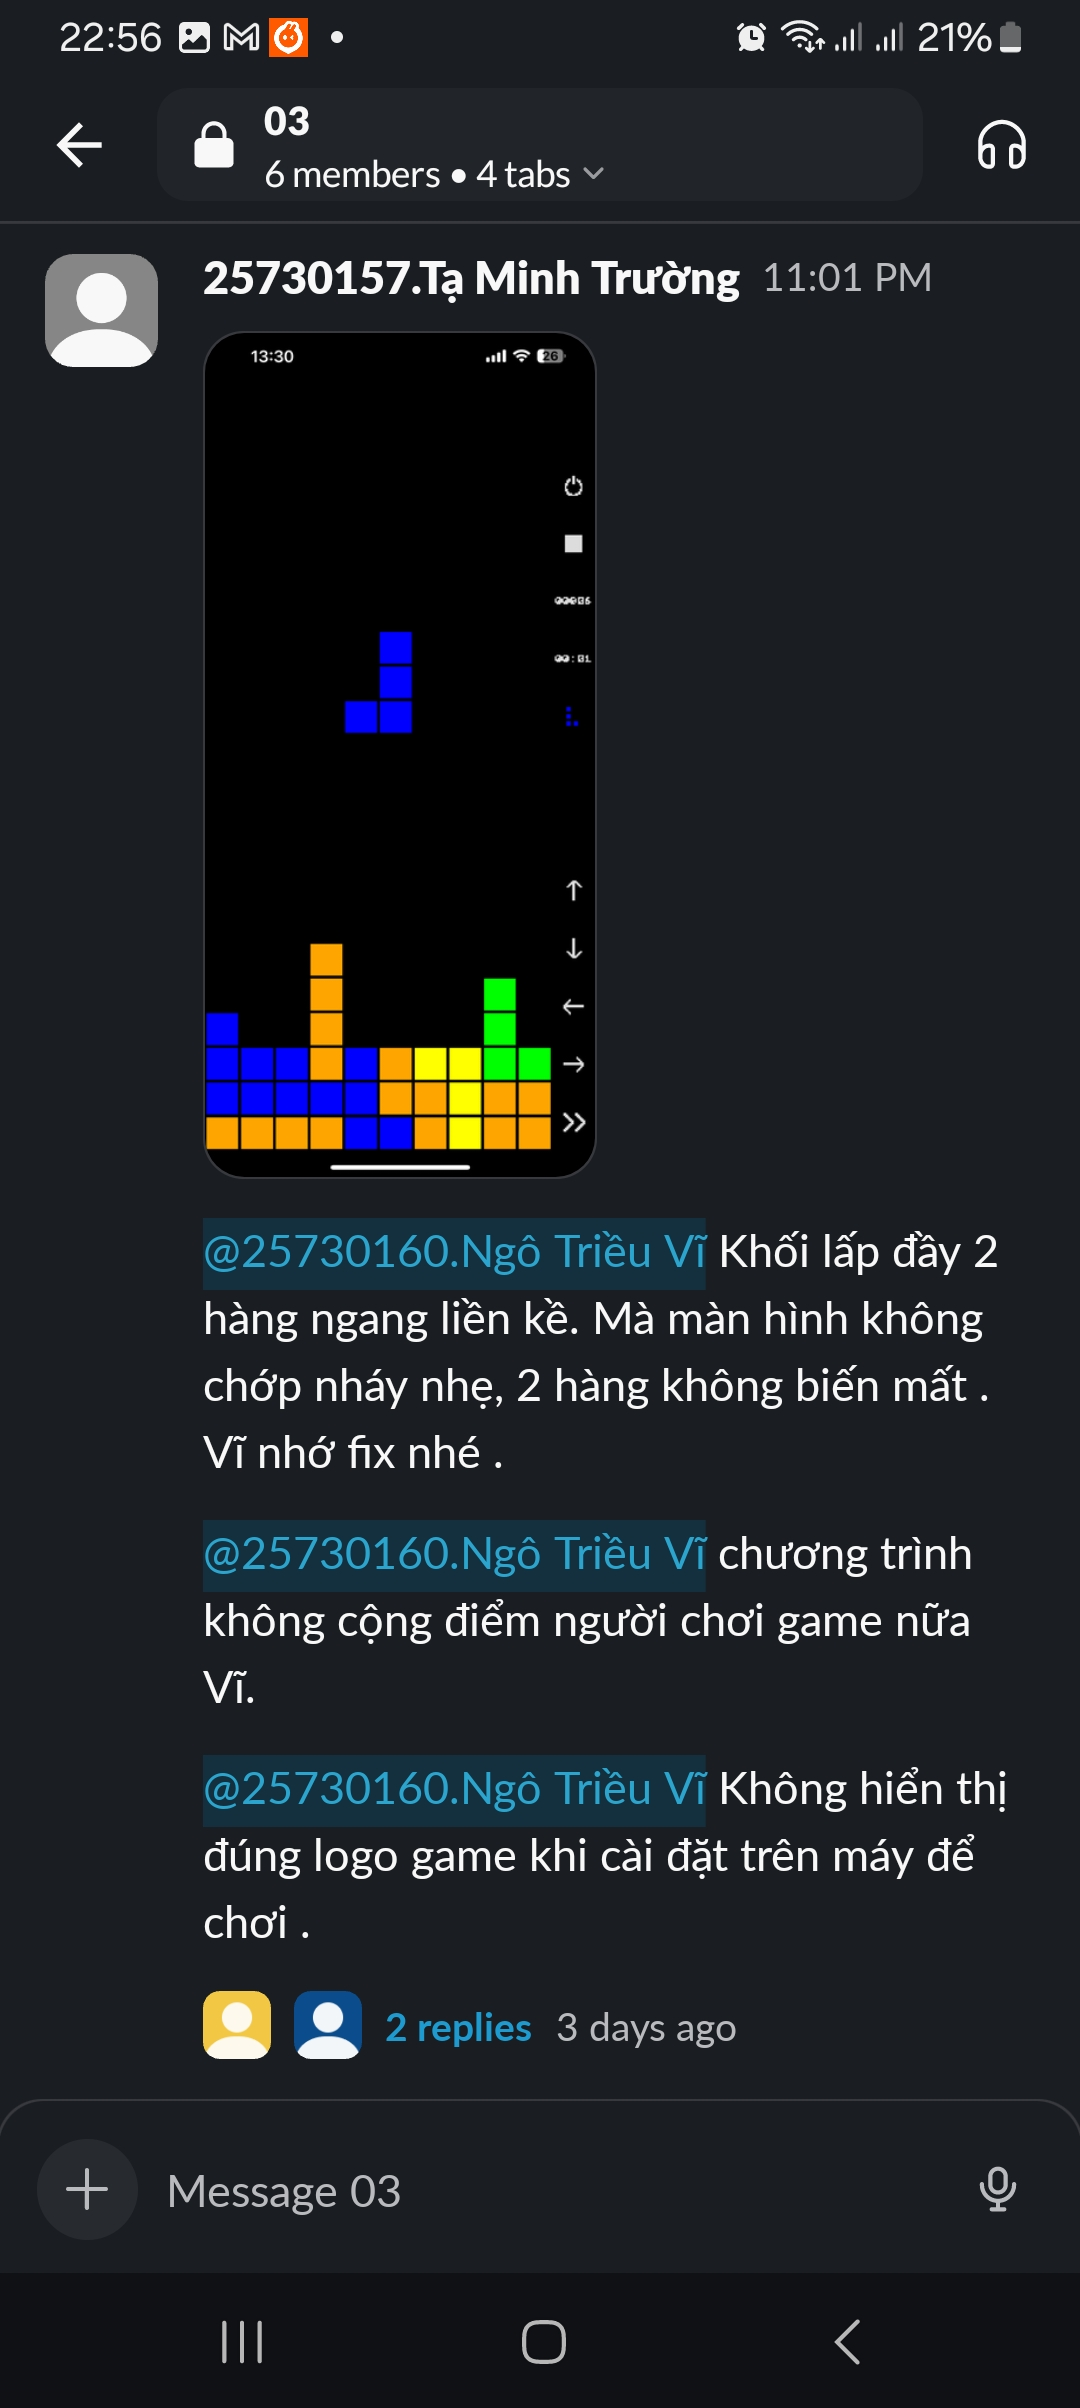
\includegraphics[width=\linewidth]{appendix-04-slack-truongtm}
        \vspace{5pt}
        \textit{\small Hình 4.1: Tester báo lỗi}
    \end{minipage}\hfill
    \begin{minipage}[t]{0.24\textwidth}
        \vspace{0pt}
        \centering
        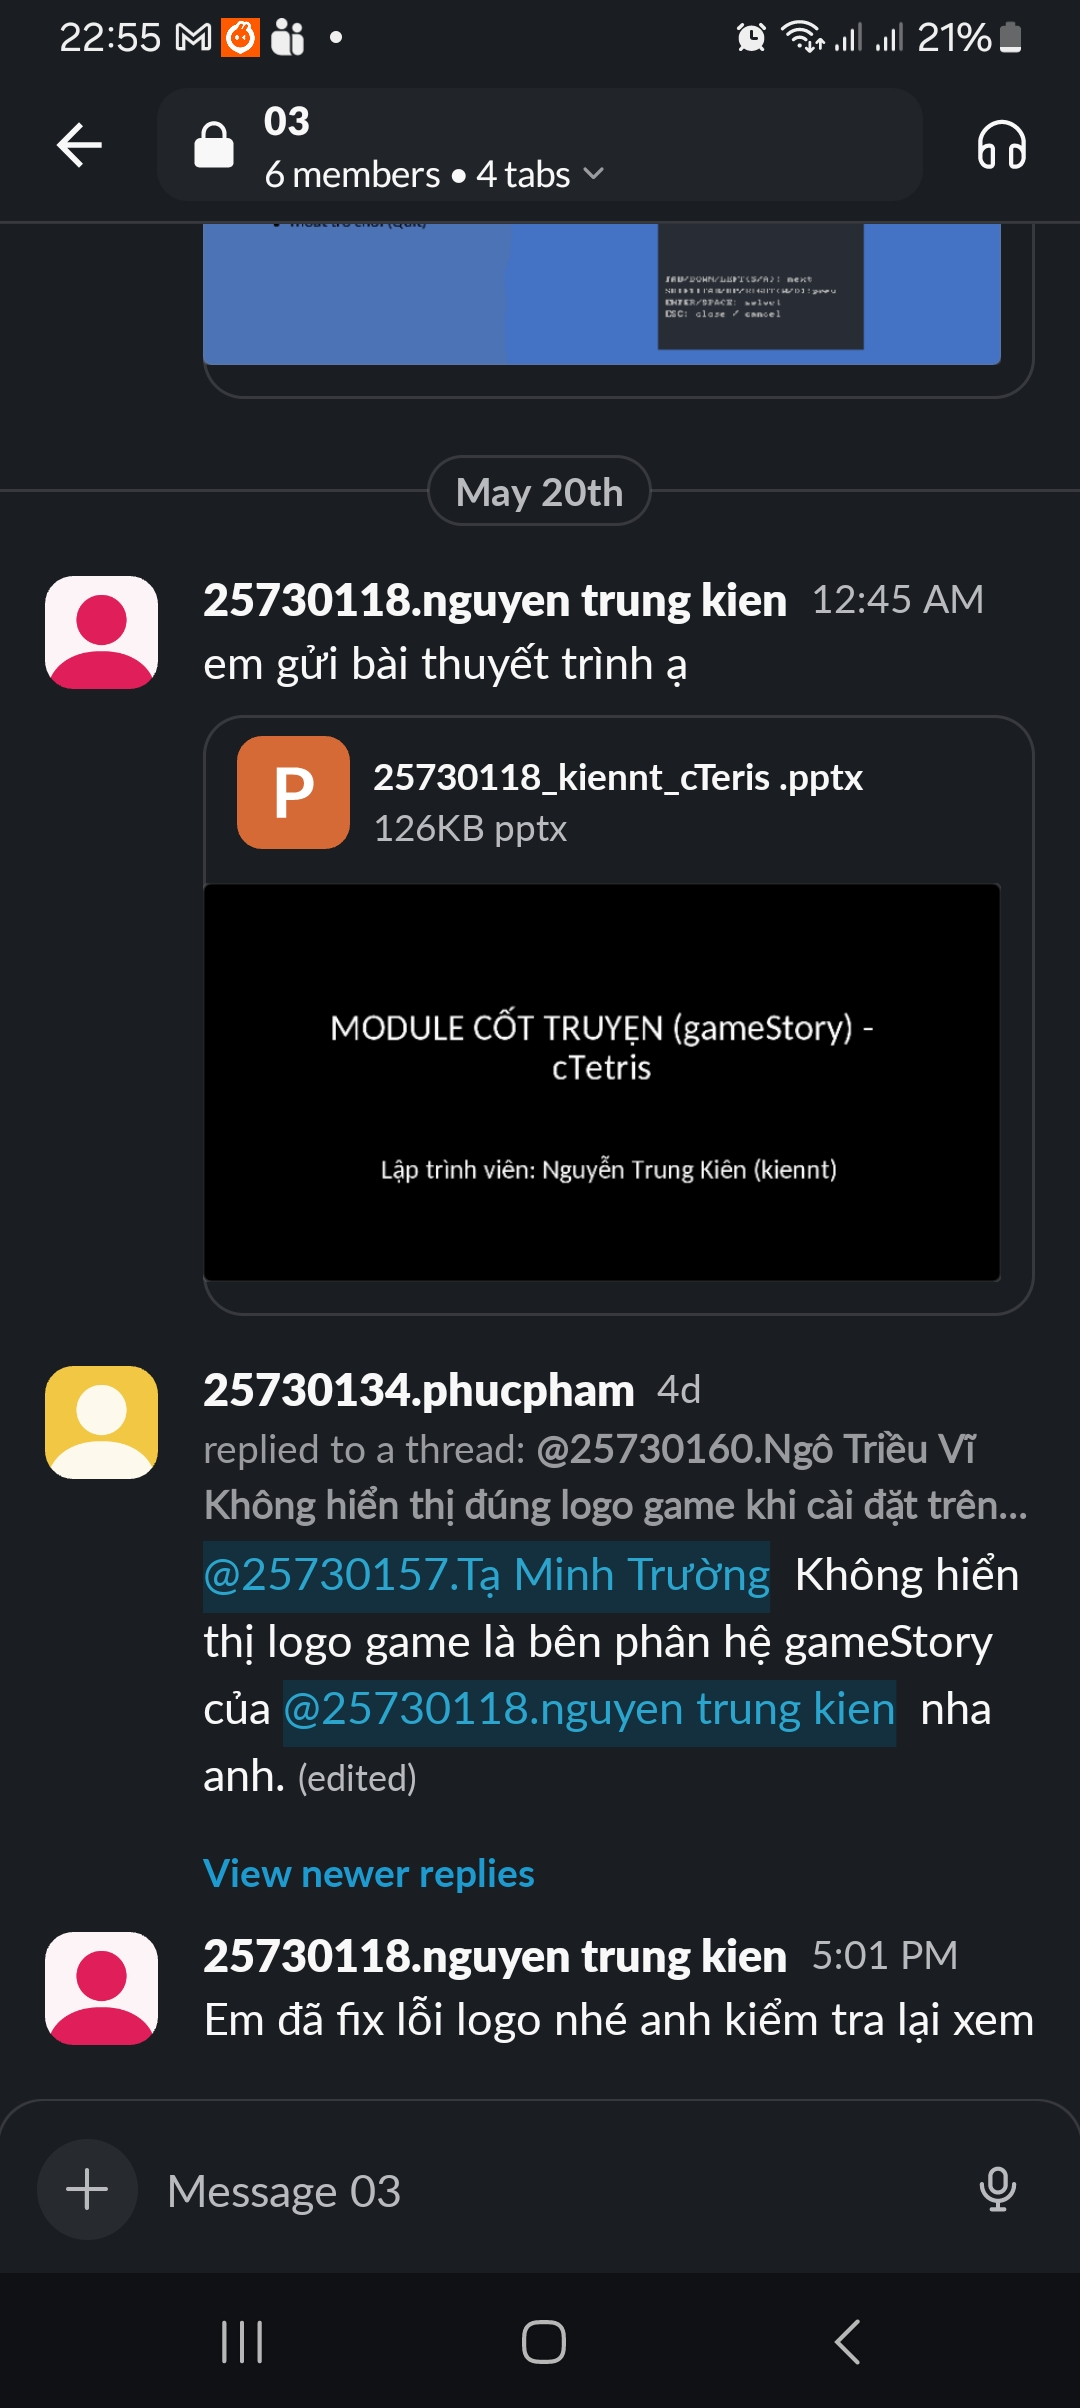
\includegraphics[width=\linewidth]{appendix-04-slack-kiennt}
        \vspace{5pt}
        \textit{\small Hình 4.2: Giao tiếp xử lý lỗi}
    \end{minipage}\hfill
    \begin{minipage}[t]{0.24\textwidth}
        \vspace{0pt}
        \centering
        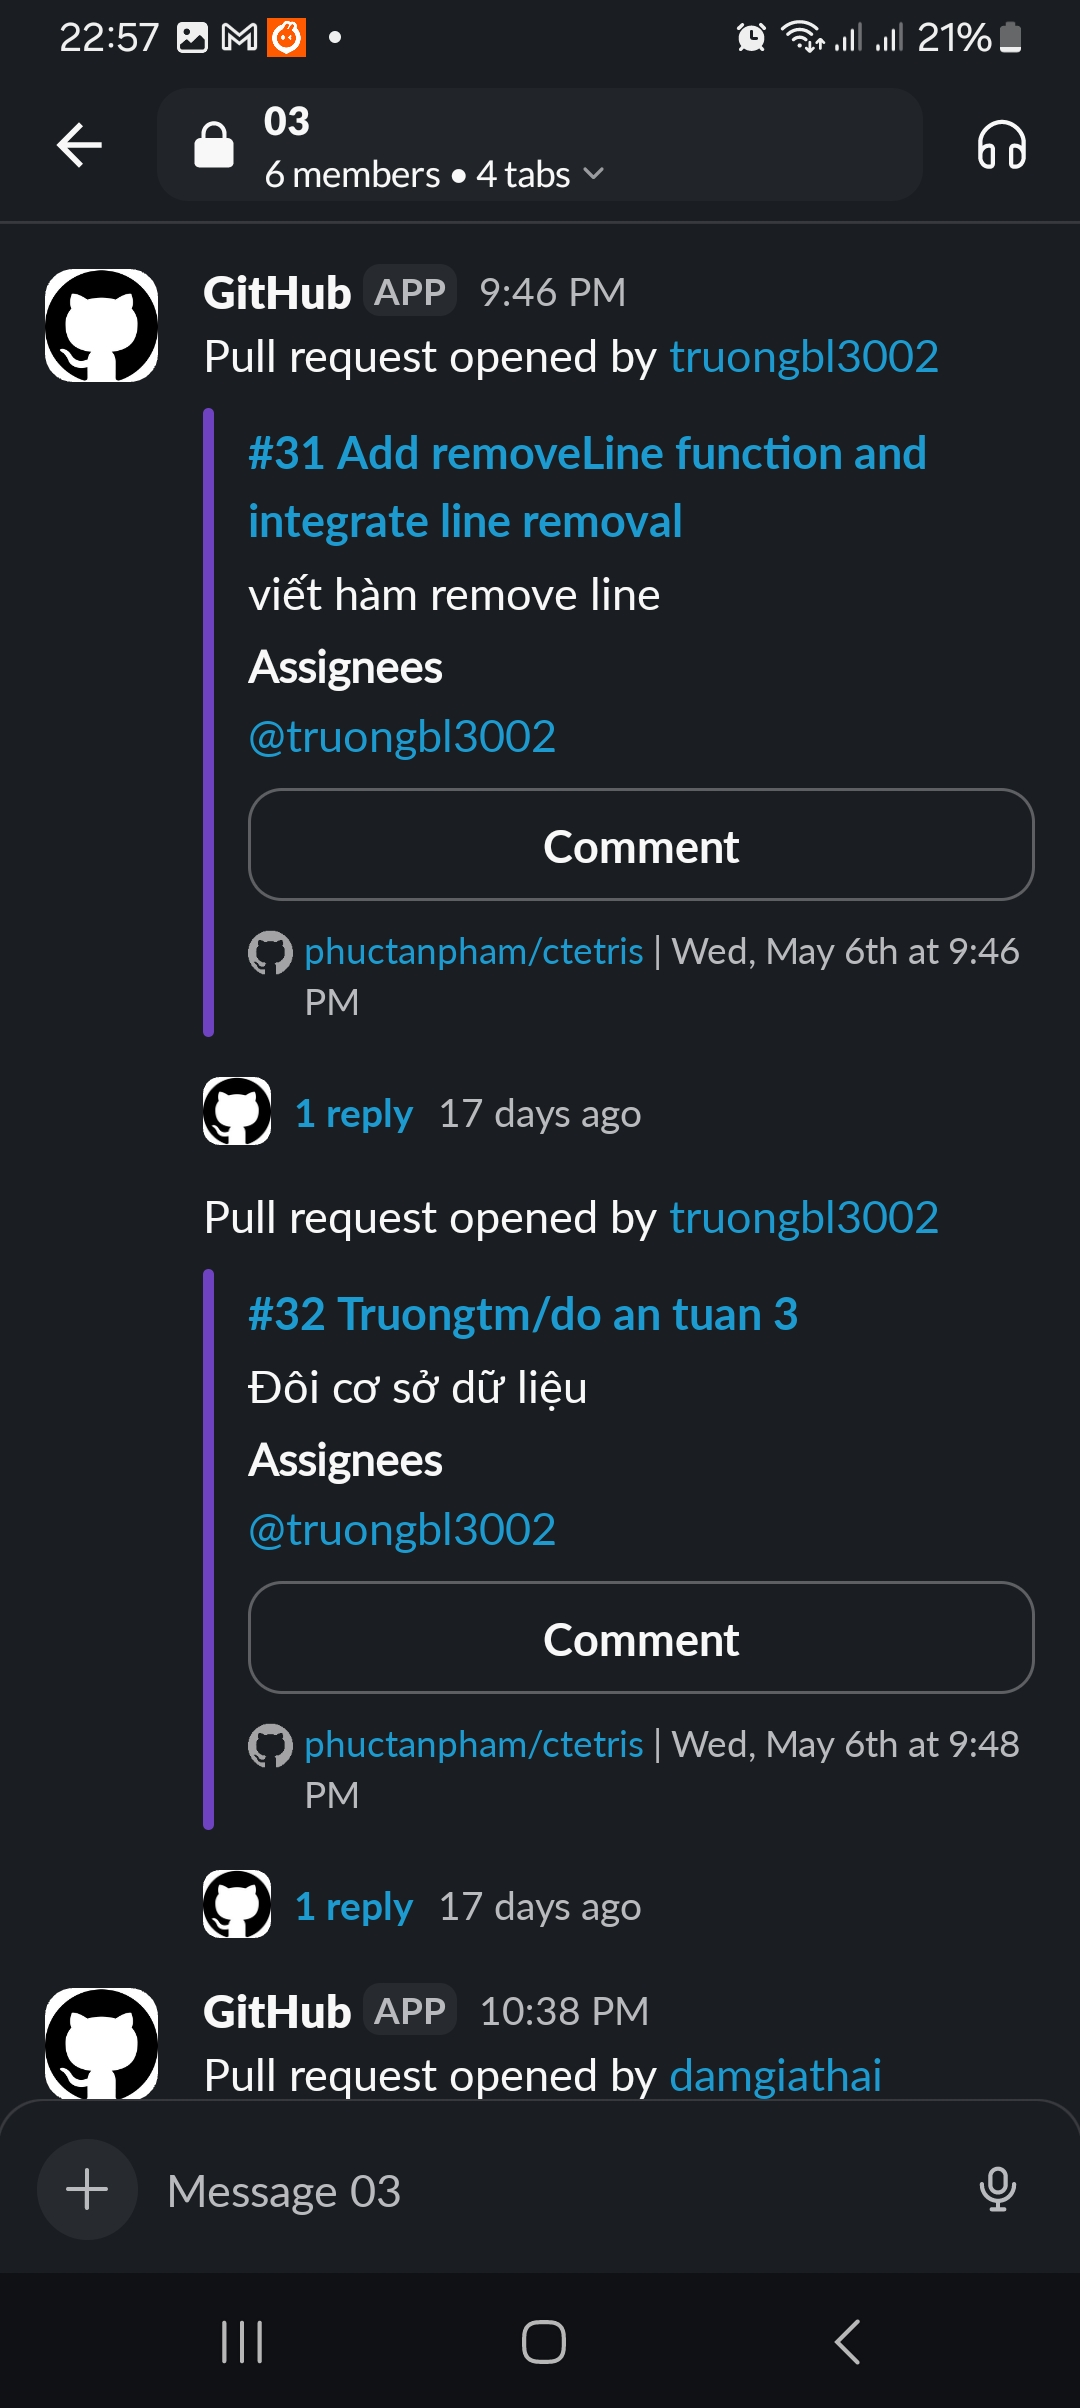
\includegraphics[width=\linewidth]{appendix-04-slack-thaidg}
        \vspace{5pt}
        \textit{\small Hình 4.3: Slack cảnh báo PR mới}
    \end{minipage}\hfill
    \begin{minipage}[t]{0.24\textwidth}
        \vspace{0pt}
        \centering
        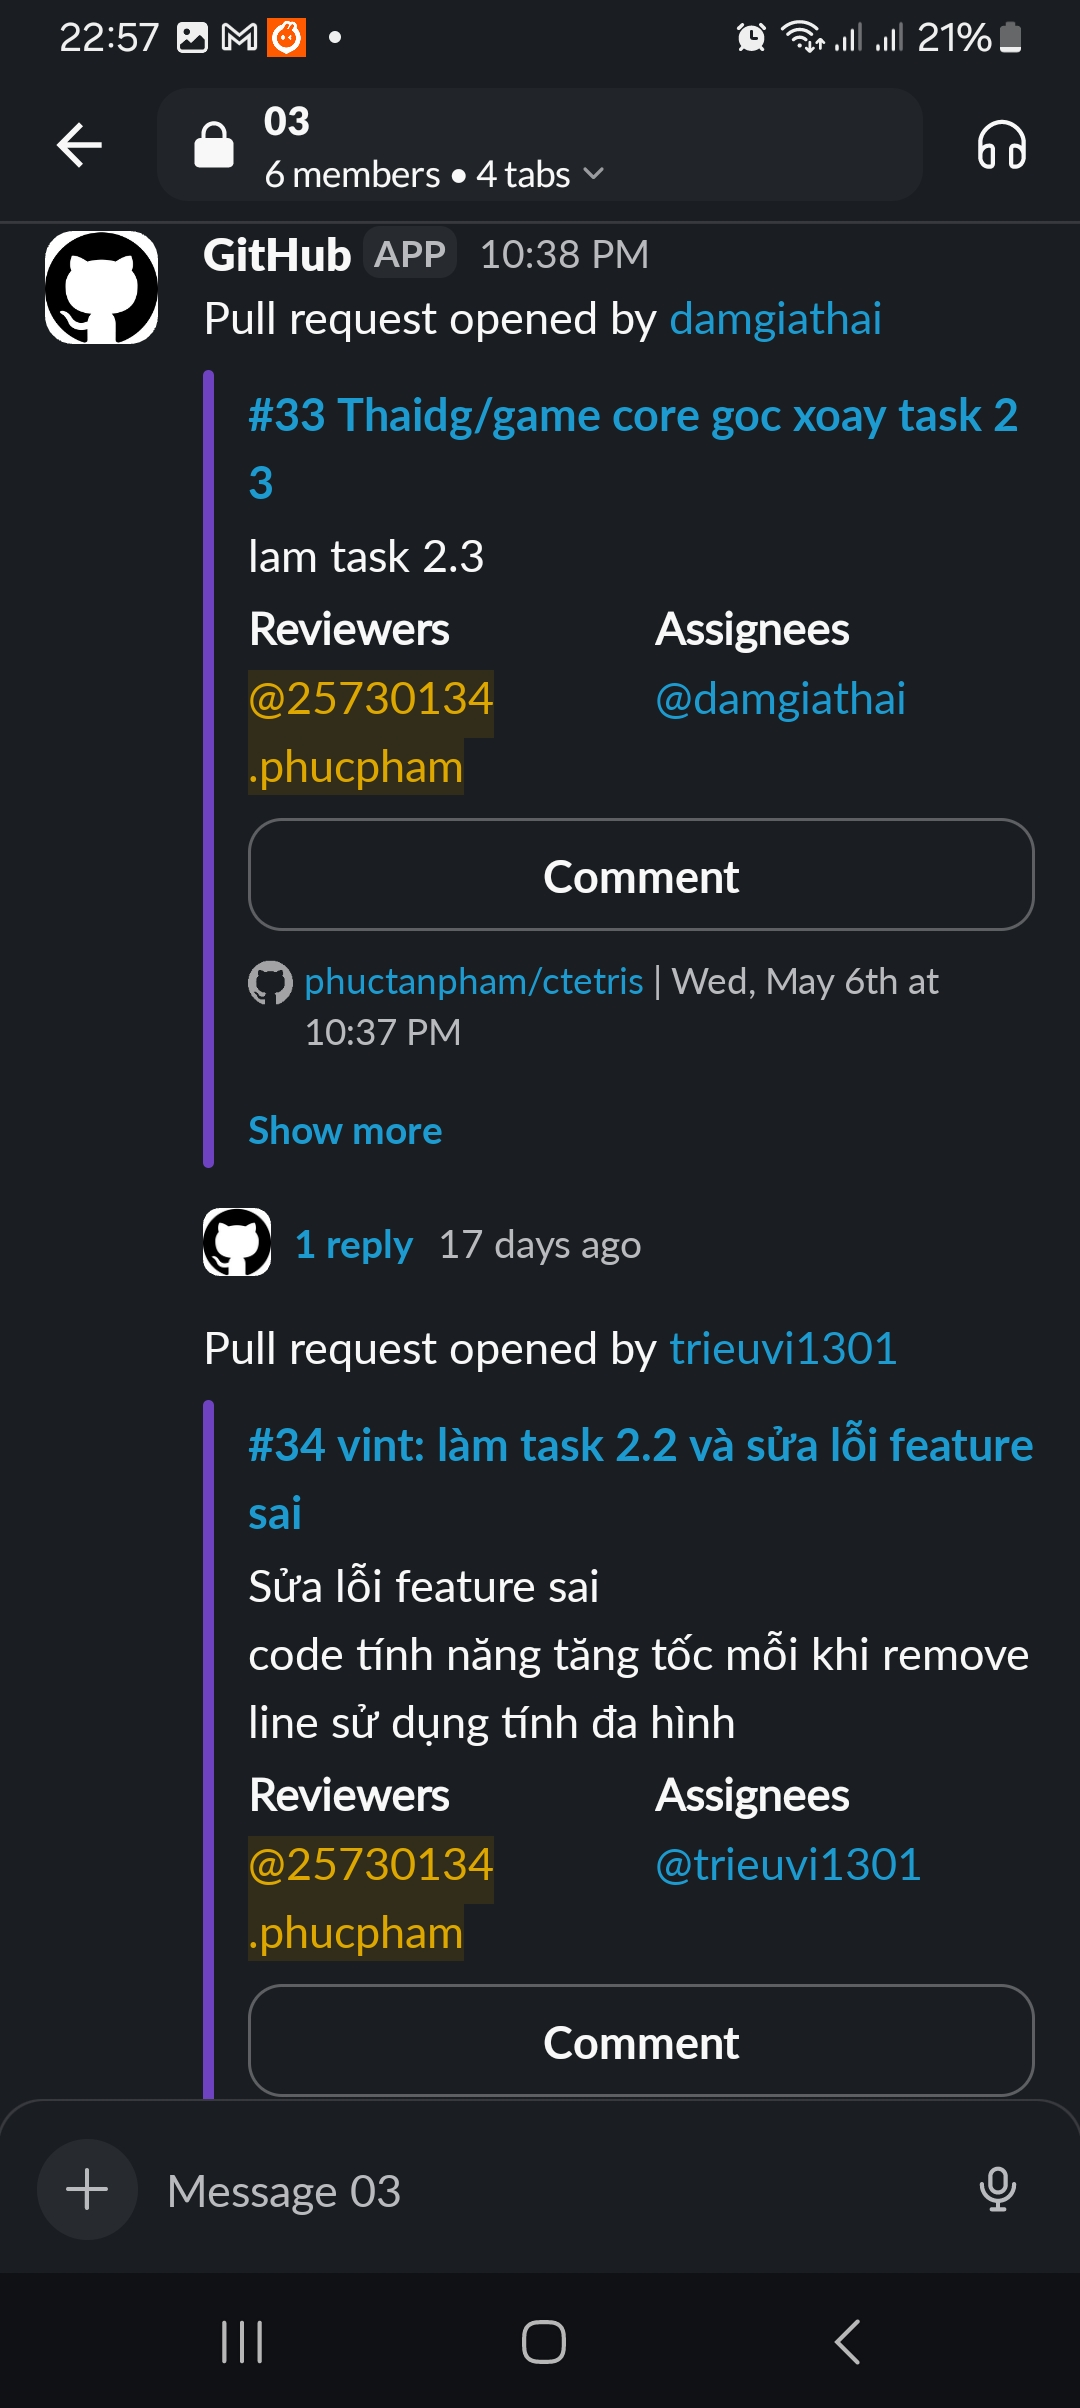
\includegraphics[width=\linewidth]{appendix-04-slack-vint}
        \vspace{5pt}
        \textit{\small Hình 4.4: Phối hợp pull code để sửa conflict}
    \end{minipage}
\end{figure}

\subsection*{G. Tích hợp đồng bộ giữa Slack và Trello}
Nhằm tối ưu hóa quy trình quản lý và theo dõi tiến độ dự án, nhóm đã thiết lập liên kết tự động giữa nền tảng quản lý công việc (Trello) và không gian giao tiếp (Slack). Khi có bất kỳ thẻ (card) công việc nào được tạo mới, cập nhật trạng thái hoặc hoàn thành trên Trello, hệ thống sẽ tự động đẩy thông báo về kênh thảo luận chung trên Slack. Điều này giúp toàn bộ thành viên nắm bắt tình hình dự án theo thời gian thực mà không cần phải chuyển đổi qua lại giữa các ứng dụng.

\begin{figure}[H]
    \centering
    \begin{minipage}[t]{0.48\textwidth}
        \vspace{0pt}
        \centering
        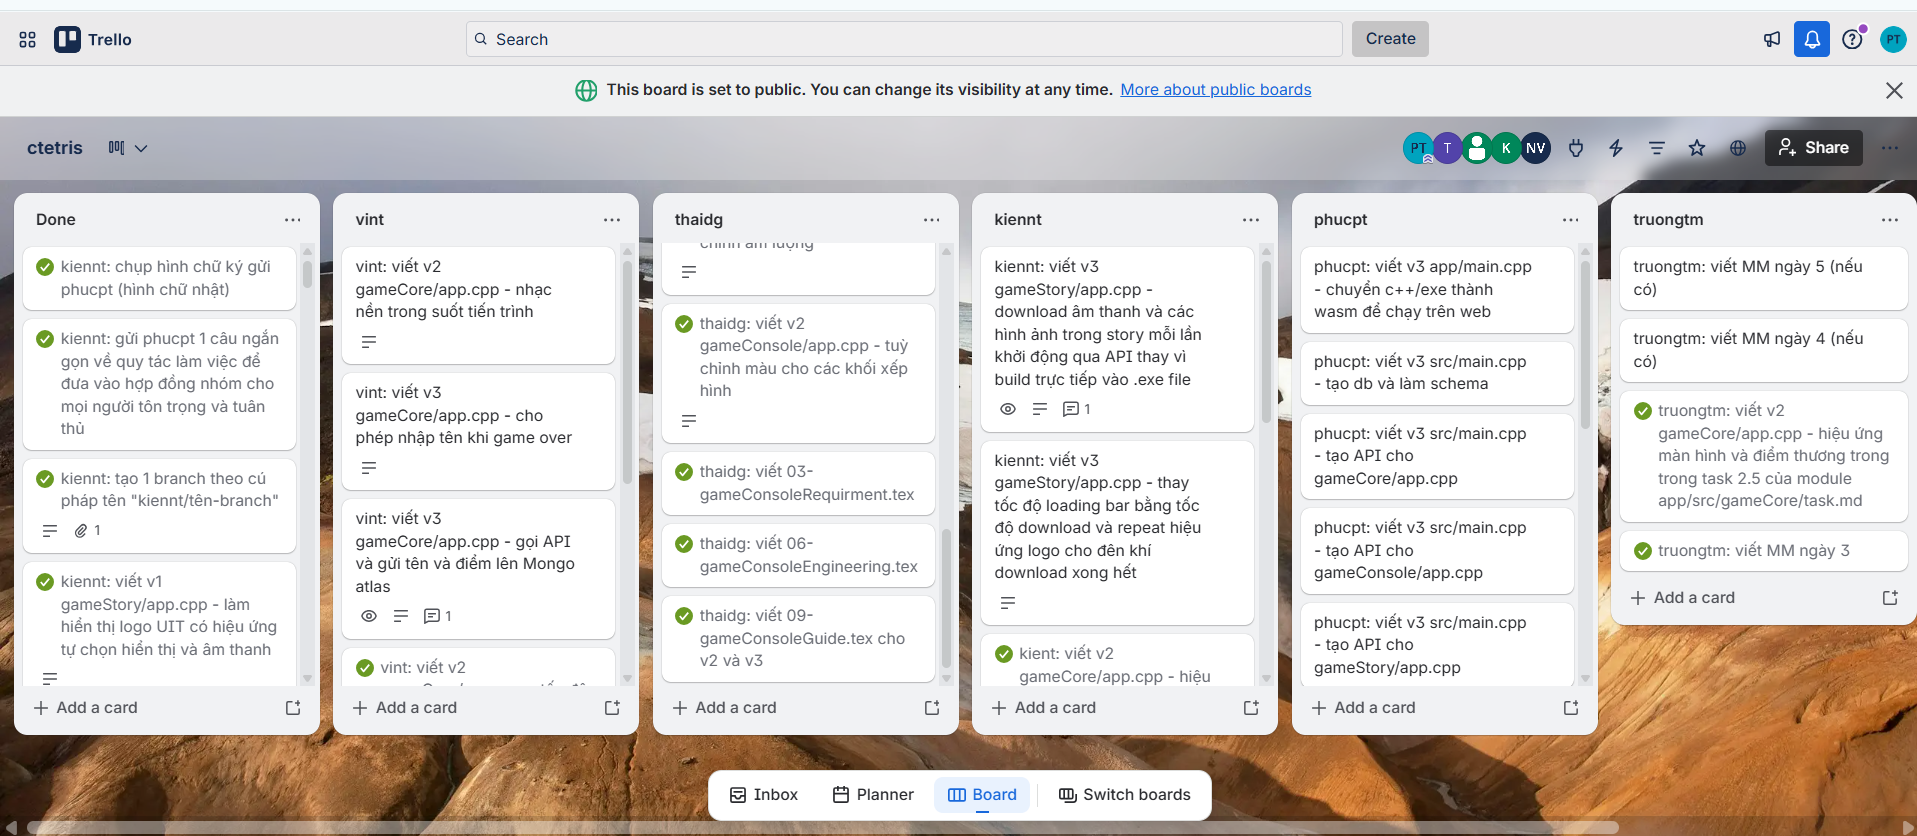
\includegraphics[width=\linewidth]{appendix-04-trello}
        \vspace{5pt}
        \textit{\small Hình 4.5: Quản lý, phân công và cập nhật Task trên Trello}
    \end{minipage}\hfill
    \begin{minipage}[t]{0.48\textwidth}
        \vspace{0pt}
        \centering
        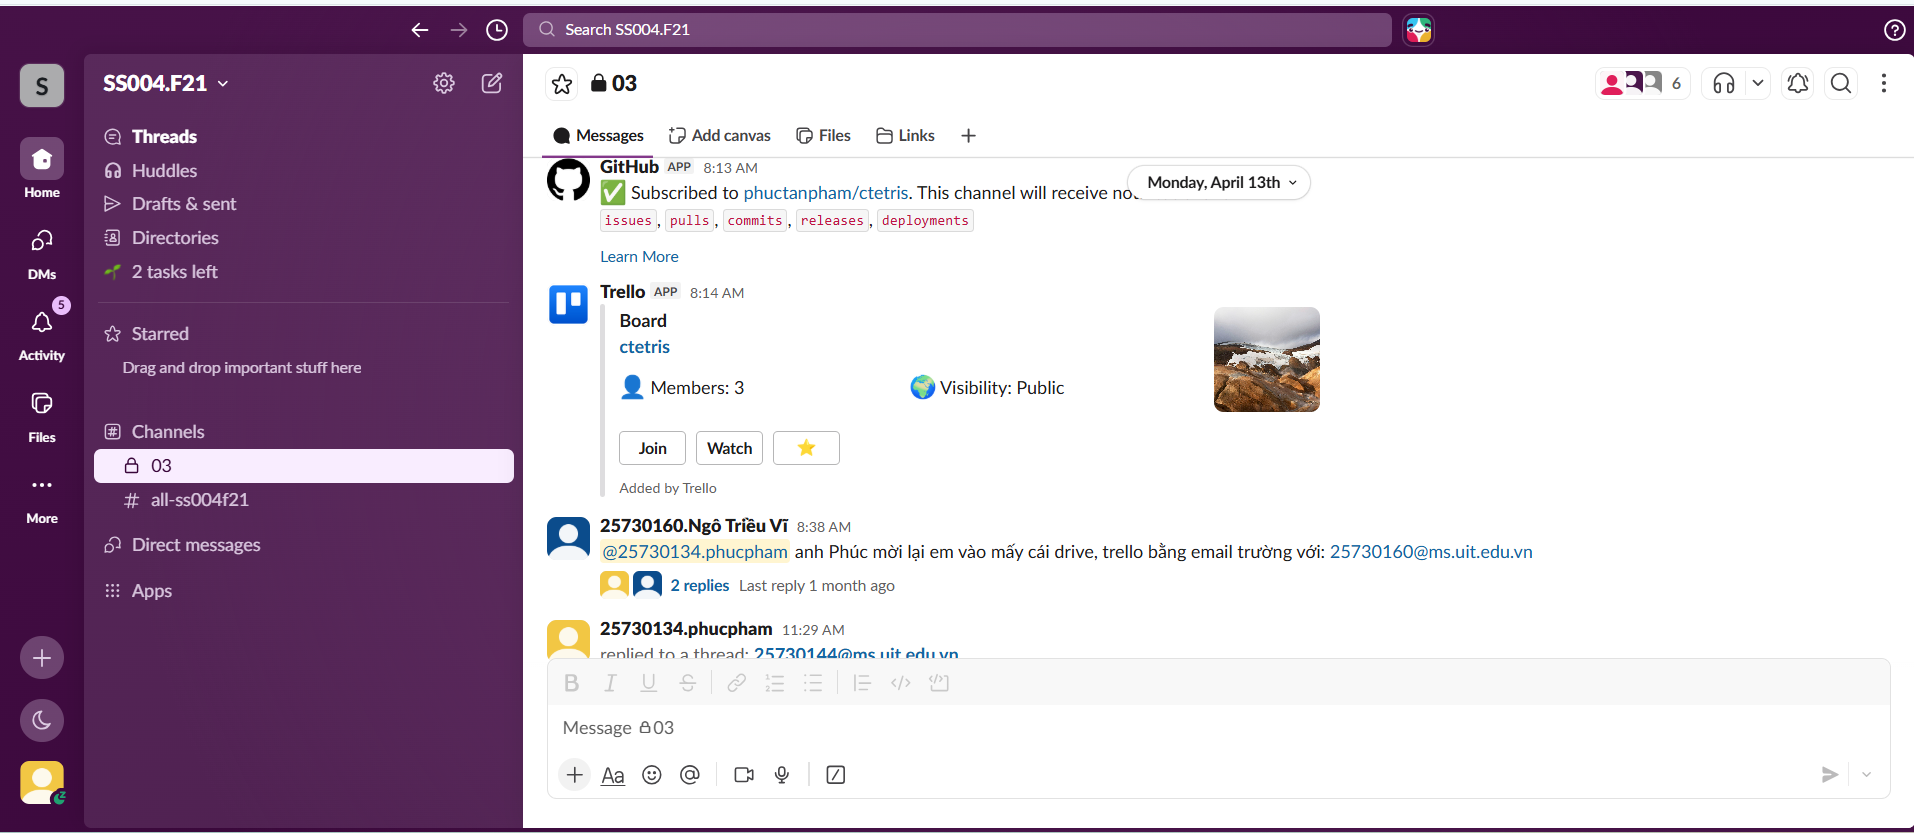
\includegraphics[width=\linewidth]{appendix-04-slack}
        \vspace{5pt}
        \textit{\small Hình 4.6: Thông báo tiến độ tự động đồng bộ sang Slack}
    \end{minipage}
\end{figure}

\label{LastPageTeamConflictSolving}
\end{document}